This is the chapter where i will put all the works related to the a successful testing

% \begin{abstract}
%     The past decade witnessed the inclusion of power measurements to evaluate the energy efficiency of software systems, thus making energy a prime indicator along with performance.
%     Nevertheless, measuring the energy consumption of a software system remains a tedious task for practitioners.
%     In particular, the energy measurement process may be subject to a lot of variations that hinder the relevance of potential comparisons.
%     While the state of the art mostly acknowledged the impact of hardware factors (chip printing process, CPU temperature), this paper investigates the impact of controllable factors on these variations.
%     More specifically, we conduct an empirical study of multiple controllable parameters that one can easily tune to tame the energy consumption variations when benchmarking software systems.

%     To better understand the causes of such variations, we ran more than a $1,000$ experiments on more than $100$ nodes with different workloads and configurations.
%     The main factors we studied encompass: experimental protocol, CPU features (C-states, Turbo~Boost, core pinning) and generations, as well as the operating system.
%     Our experiments showed that, for some workloads, it is possible to tighten the energy variation by up to $30\times$.
%     Finally, we summarize our results as guidelines to tame energy consumption variations.
%     We argue that the guidelines we deliver are the minimal requirements to be considered prior to any energy efficiency evaluation.
% \end{abstract}


% \section{Introduction}
%\lettrine[nindent=0em,lines=3]{C} 
% To conduct robust evaluations, practitioners often try to ensure reproducible environmental conditions in order to properly benchmark their software systems.
% 
% Recently, the research community has been investigating typical "crimes" in systems benchmarking and established guidelines for conducting robust and reproducible evaluations~\cite{DBLP:journals/corr/abs-1801-02381}.

% In theory, using identical CPU, same memory configuration, similar storage and networking capabilities, should favour reproducible experiments.
% However, when it comes to measuring the energy consumption of a system, applying acknowledged guidelines and carefully repeating the same benchmark can nonetheless lead to different energy footprints not only on homogeneous nodes, but even within a single node.
% This difference---also called \emph{energy variation} (EV)---has become a serious threat to the accuracy of experimental evaluations.

% Figure~\ref{fig:motivation} illustrates this variation problem as a violin plot of $20$ executions of the benchmark \emph{Conjugate Gradient} (\textsf{CG}) taken from the \emph{NAS Parallel Benchmarks} (NBP) suite~\cite{Bailey:1991:NPB:125826.125925}, on $4$ nodes of an homogeneous cluster (the cluster \textsf{Dahu} described in Table~\ref{table:g5k}) at 50\,\% workload.
% One can observe a large variation of the energy consumption, not only among homogeneous nodes, but also at the scale of a single node, reaching up to $25\,\%$ in this example.

% \begin{figure}%[!htb]
%     \center{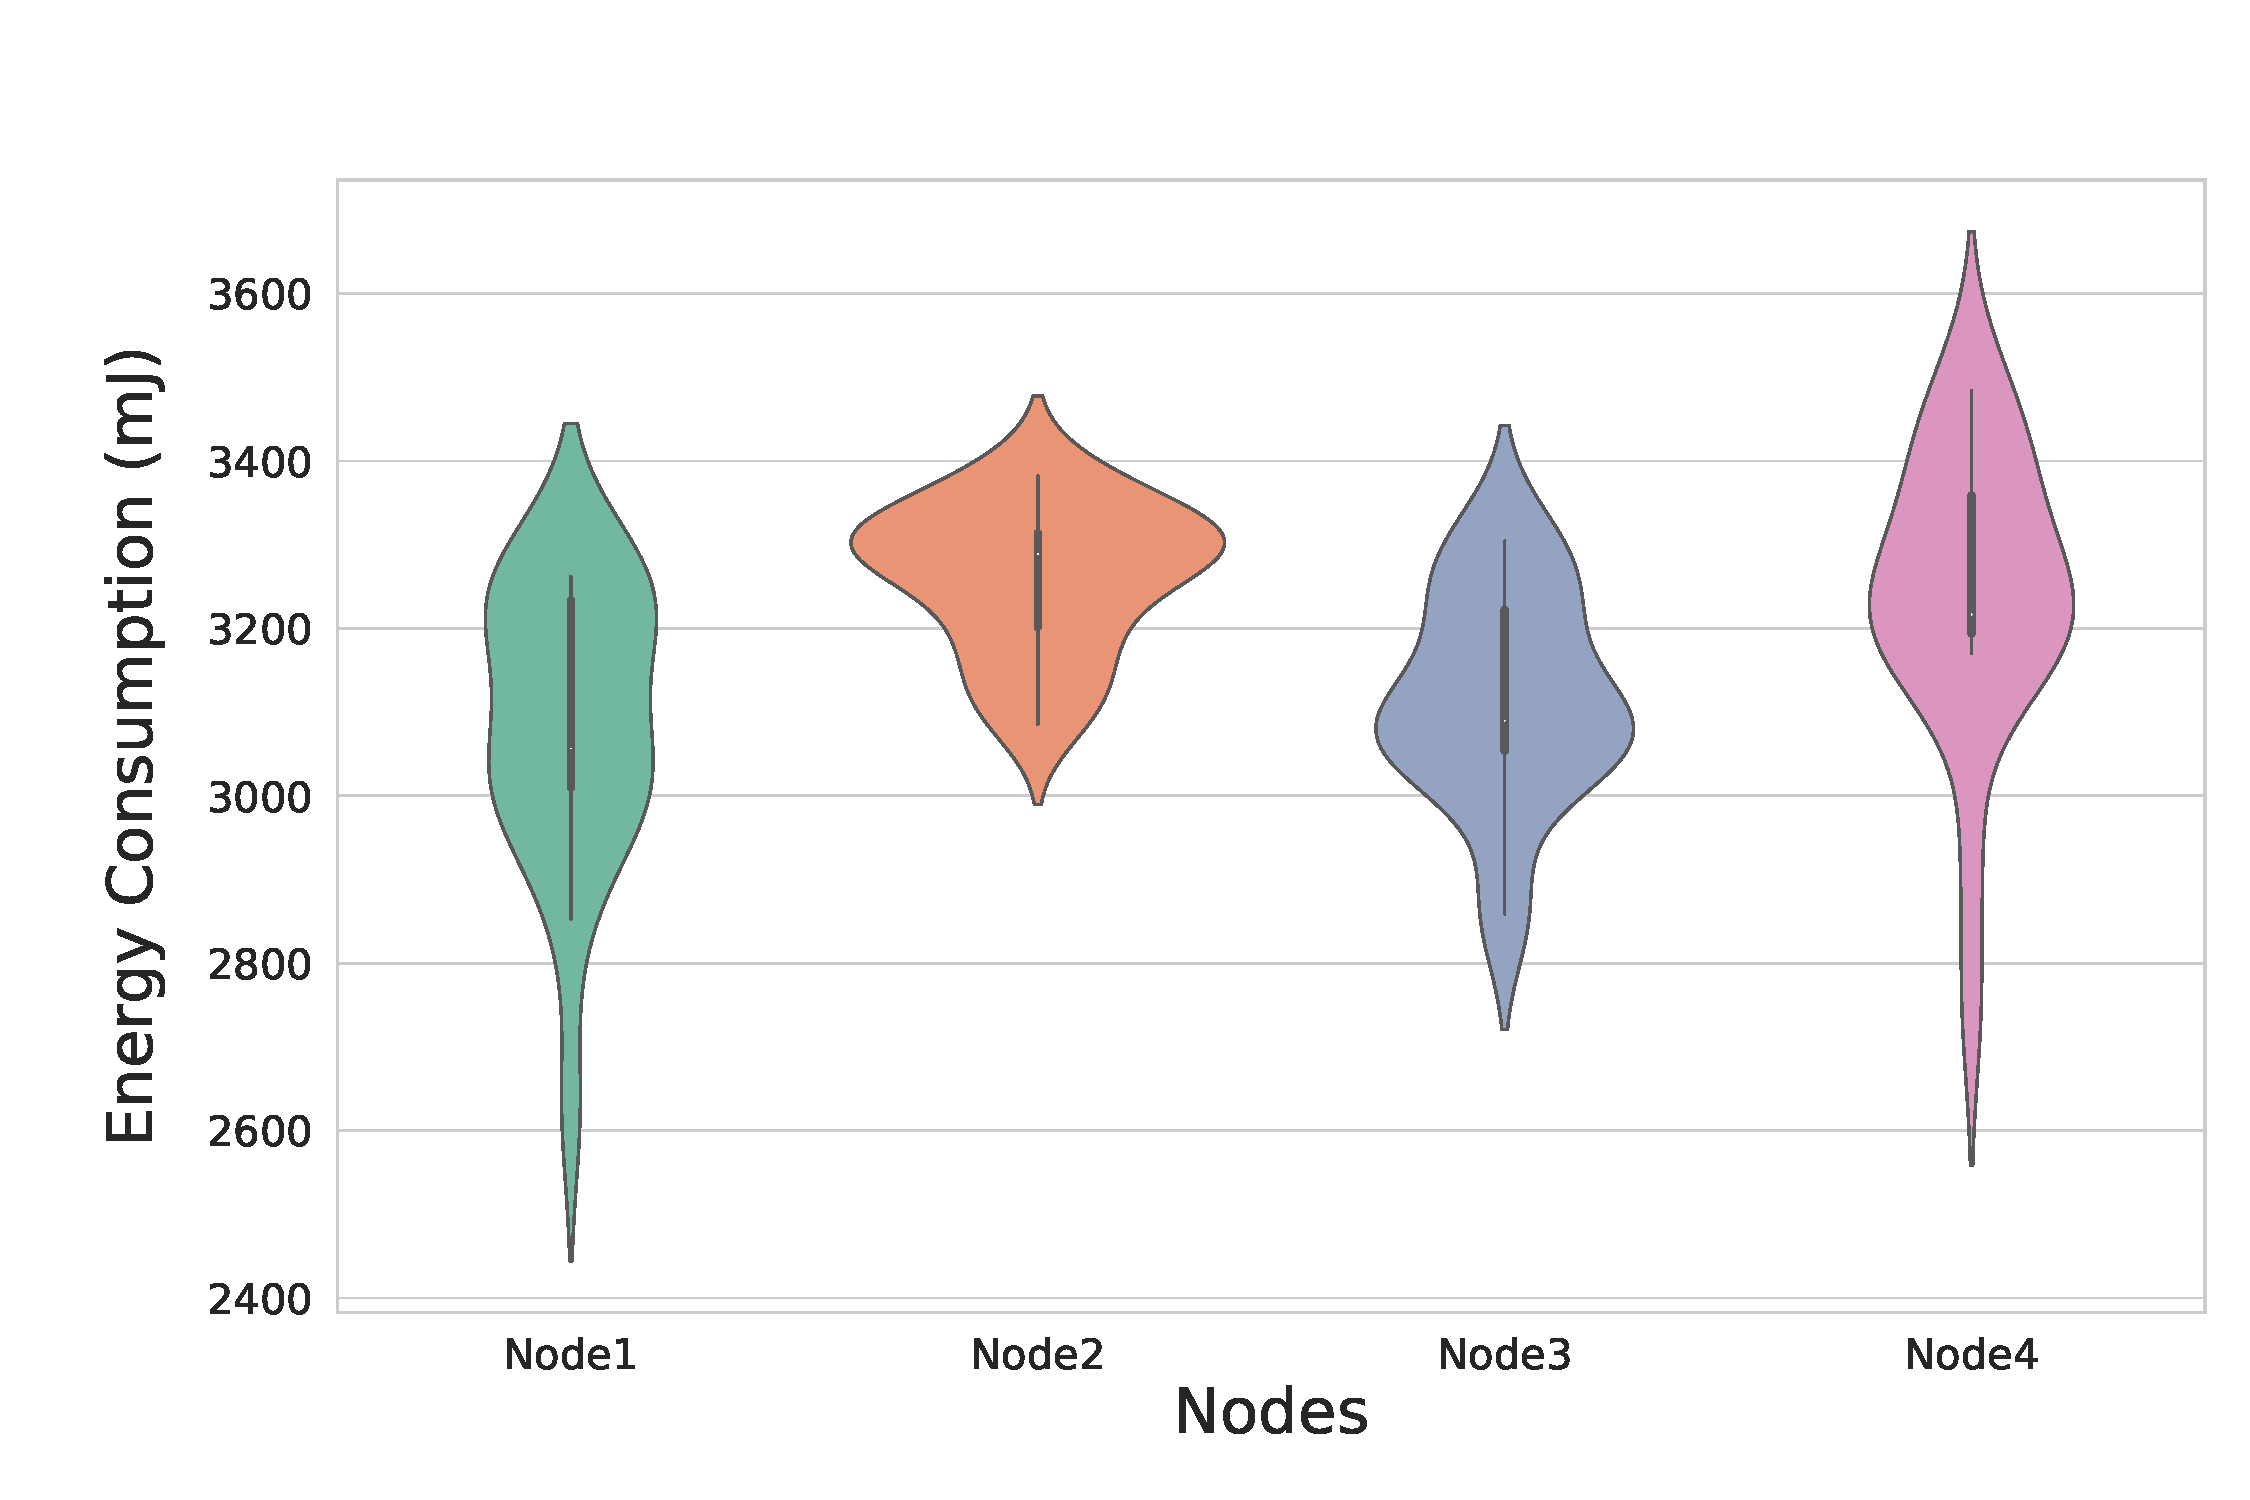
\includegraphics[width=.9\linewidth]{imgs/motivation}}
%     \caption{CPU energy variation for the benchmark \textsf{CG}}\label{fig:motivation}
% \end{figure}


Most of the state of the art has been investigating this power consumption issue from a hardware perspective~\cite{borkar_designing_2005,tschanz_adaptive_2002} and reported that the causes of such energy variations are CMOS manufacturing process of transistors in a chip, differences in node assembly and data center hot spots.
Additionally, \cite{heinrich_predicting} described it as a combination of parameters, mentioning a list of candidate factors, such as the thermal effect or the CPU frequency, but failing to deliver a deeper analysis of these factors.

Unfortunately, hardware factors can be hardly tuned to tame the energy variation that can be observed in systems benchmarking.
For example, managing the CPU temperature or a server position in a cluster, are not actions that one can easily do, especially on the modern data centers and cloud platforms.
Therefore, the goal of this paper is to investigate the spectrum of factors that can cause or increase the variability of energy consumption in systems benchmarking, and to propose effective guidelines to control such factors in order to mitigate this variability.
% While this paper does not question the benefits of established CPU features, like C-states or Turbo~Boost, it delivers a deeper analysis of the effects they may introduce on a wide set of experiments and nodes.
% By quantifying potential energy variations induced by controllable factors, we intend to identify the proper configurations that minimize energy variations, depending on the workload characteristics.
% These guidelines aim at supporting practitioners in conducting robust system benchmarks and reporting reproducible energy consumption, rather than recommending production-scale practices or solutions to reduce the power consumption of a given system.
% 
% The key contributions of this paper can therefore be summarized as:
% \begin{enumerate}
%     \item Providing a better understanding of the energy variation, by using different generations of CPU deployed in $4$ clusters with more than $100$ physical nodes, and by considering existing systems benchmarks with diverse workloads;
%     \item Identifying controllable factors that contribute to the variation in CPU energy consumption, comparing them against the state of the art, and completing them with other uncovered assumptions;
%     \item Reporting on some guidelines on how to conduct reproducible experiments with less energy variations;
%     \item Discussing the differences between inter-nodes and intra-nodes variations.
% \end{enumerate}

%\paragraph{}
% The remainder of this paper is organized as follows.
% Section~\ref{sec:related_work} discusses the related works in the area of power measurements.
% Section~\ref{sec:research_qs} formalizes our research questions.
% Section~\ref{sec:setup} reports on the experimental setup (hardware, benchmarks, tools and methodology) we used in this work.
% Section~\ref{sec:parameters} analyzes the causes of the variations we observed along experiments.
% Finally, we discuss the results of the different experimented factors, and their impact on the energy variation in Section~\ref{sec:guidelines}, while Sections~\ref{sec:threats} \&~\ref{sec:conclusion} cover the validity threats and our conclusions, respectively.

%------------------------------------------------
\section{Related Work}\label{sec:related_work}
In this section, we review the state of the art in the domain of energy consumption analysis.
In particular, one can observe that several studies considered the evaluation of the processor variation while executing the same workload, in particular to test distributed applications running in homogeneous clusters.

\paragraph{Studying Hardware Factors.}

This variation has often been related to the manufacturing process~\cite{coles_comparing_2014}, but has also been a subject of many studies, considering several aspects that could impact and vary the energy consumption across executions and on different chips.
On the one hand, the correlation between the processor temperature and the energy consumption was one of the most explored paths.
Kistowski~\emph{et~al.} showed in~\cite{joakim_v_kisroski_variations_2016} that identical processors can exhibit significant energy consumption variation with no close correlation with the processor temperature and performance.
On the other hand, the authors of~\cite{wang_potential_2018} claimed that the processor thermal effect is one of the most contributing factors to the energy variation, and the correlation between the CPU temperature and the energy consumption variation is very tight.

\note{add the corelation value}

This makes the processor temperature a delicate factor to consider while comparing energy consumption variations across a set of homogeneous processors.%, but also, if a same workload can cause the CPUs to reach different temperatures.

The ambient temperature was also discussed in many papers as a candidate factor for the energy variation of a processor.
In~\cite{ranka_energy_2009}, the authors claimed that energy consumption may vary due to fluctuations caused by the external environment.
These fluctuations may alter the processor temperature and its energy consumption.
However, the temperature inside a data center does not show major variations from one node to another.
In~\cite{el_mehdi_diouri_your_2013}, El~Mehdi~Dirouri~\emph{et~al.} showed that switching the spot of two servers does not affect their energy consumption.
Moreover, changing hardware components, such as the hard drive, the memory or even the power supply, does not affect the energy variation of a node, making it mainly related to the processor.
This result was recently assessed by~\cite{wang_potential_2018}, where the rack placement and power supply introduced a maximum of $2.8\,\%$ variation in the observed energy consumption.

Beyond hardware components, the accuracy of power meters has also been questioned.
Inadomi~\emph{et~al.}~\cite{inadomi_analyzing_2015} used three different power measurement tools: RAPL, Power Insight\footnote{\url{https://www.itssolution.com/products/trellis-power-insight-application}} and BGQ EMON.
All of the three tools recorded the same $10\,\%$ of energy variation, that was supposedly related to the manufacturing process.
%% this is to prove that the problem is REAL !!! 
\paragraph{Mitigating Energy Variations.}
Acknowledging the energy variation problem on processors, some papers proposed contributions to reduce and mitigate this variation.
In~\cite{inadomi_analyzing_2015}, the authors introduced a variation-aware algorithm that improves application performance under a power constraint by determining module-level (individual processor and associated DRAM) power allocation, with up to $5.4\times$ speedup.
The authors of~\cite{hammouda_noise-tolerant_2015} proposed parallel algorithms that tolerate the variability and the non-uniformity by decoupling per process communication over the available CPU.
Acun~\emph{et~al.}~\cite{acun_variation_2016} found out a way to reduce the energy variation on Ivy~Bridge and Sandy~Bridge processors, by disabling the Turbo~Boost feature to stabilize the execution time over a set of processors.
They also proposed some guidelines to reduce this variation by replacing the old slow chips, by load balancing the workload on the CPU cores and leaving one core idle.
They claimed that the variation between the processor cores is insignificant.
In~\cite{chasapis_runtime-guided_2016}, the researchers showed how a parallel system can be used to deal with the energy variation by compensating the uneven effects of power capping.

In~\cite{marathe_empirical_2017_m}, the authors highlight the increase of energy variation across the latest Intel micro-architectures by a factor of $4$ from Sandy~Bridge to Broadwell, a $15\,\%$ of run-to-run variation within the same processor and the increase of the inter-cores variation from $2.5\,\%$ to $5\,\%$ due to hardware-enforced constraints, concluding with some recommendations for Broadwell usage, such as running one hyper-thread per core.
\note{this might be interesting for greeFaaS}

% \paragraph{Objective.}
% The aim of our paper is not to reproduce all the exposed results and explored paths.
% Instead, we intend to check some of these results on latest hardware components, and to consider new potential controllable factors that could also contribute to the energy variation.
% We also aim to provide practitioners with guidelines to conduct robust experiments in a controlled environment, thus reducing the variation overhead to share trustable results and build credible comparisons.

\section{Research Questions}\label{sec:research_qs}
Worth saying, we are aware that part of the energy consumption variation is due to chip manufacturing differences or some of the previously discussed enforced factors, such as the thermal effect or the servers placement.
Those parameters are often tricky to manage, as we cannot have a perfect chips manufacturing process, or assume that two identical processors have the same thermal behavior.
We will therefore focus on providing the practitioners with an empirical study of some controllable parameters that can be tuned to conduct experimental evaluations of energy consumption with less variation, especially if the practitioners do not have a physical access to the data center or BIOS configuration, which is the case on most of the modern cloud platforms and data centers.
These parameters span the choice of the benchmarking protocol, processor frequencies management, operating system tuning or some other parameters.
The authors of~\cite{heinrich_predicting} mentioned some of these potential parameters.

In this paper, we will therefore investigate the following controllable factors, which we formalize as 4 research questions:
\begin{description}
    \item[\textsc{RQ}~1:] Does the benchmarking protocol affect the energy variation?
    \item[\textsc{RQ}~2:] How important is the impact of the processor features on the energy variation?
    \item[\textsc{RQ}~3:] What is the impact of the operating system on the energy variation? and finally
    \item[\textsc{RQ}~4:] Does the choice of the processor matter to mitigate the energy variation?
\end{description}


\section{Experimental Setup}\label{sec:setup}
This section describes our detailed experimental environment, covering the clusters and nodes configuration, the benchmarks we used and justifying our experimental methodology.

\subsection{Hardware Platform}
We considered 4 distinct clusters of variable sizes and different generations of CPU, as summarized in Table~\ref{table:g5k}.
In particular, we used the Grid5000 (G5K) platform in our experiments~\cite{grid5000,margery:hal-00965708}.
G5K is a bare metal cloud platform that can be used to provision clusters of identical nodes.
In our study, we mainly used the cluster \textsf{Dahu} located in Grenoble to run most of our tests, as it has one of the newest Xeon CPUs.
We also used the clusters \textsf{Chetemi}, \textsf{Ecotype} and \textsf{Paranoia} in some of our experiments.
Table~\ref{table:g5k} describes the configurations of the clusters we considered.
% We note that each cluster is geographically independent. 

\begin{table}
    \centering
    \caption{Description of clusters included in the study}
    \label{table:g5k}
    \small
    \begin{tabular}{|l|l|r|r|}
        \hline
        \textbf{Cluster}  & \textbf{Processor}               & \textbf{Nodes} & \textbf{RAM} \\
        \hline
        \hline
        \textsf{Dahu}     & $2\times$ Intel Xeon\,Gold\,6130 & 32             & 192\,GiB     \\
        \hline
        \textsf{Chetemi}  & $2\times$ Intel Xeon\,E5-2630v4  & 15             & 768\,GiB     \\
        \hline
        \textsf{Ecotype}  & $2\times$ Intel Xeon\,E5-2630Lv4 & 48             & 128\,GiB     \\
        \hline
        \textsf{Paranoia} & $2\times$ Intel Xeon\,E5-2660v2  & 8              & 128\,GiB     \\
        \hline
    \end{tabular}
\end{table}

As most of the nodes are equipped with two sockets (physical processors), we use the acronym \textsf{CPU} or socket to designate one of the two sockets and \textsf{PU} for the operating system \emph{processing unit}.
The number of \textsf{PU} often doubles the number of available cores because of the hyper-threading support, as the OS considers 2 hyper-threads sharing the same core as 2 different \textsf{PU}.
Figure~\ref{fig:topo} illustrates a detailed topology of a node belonging to the cluster \textsf{Dahu}.

\begin{figure}%[!htb]
    \center{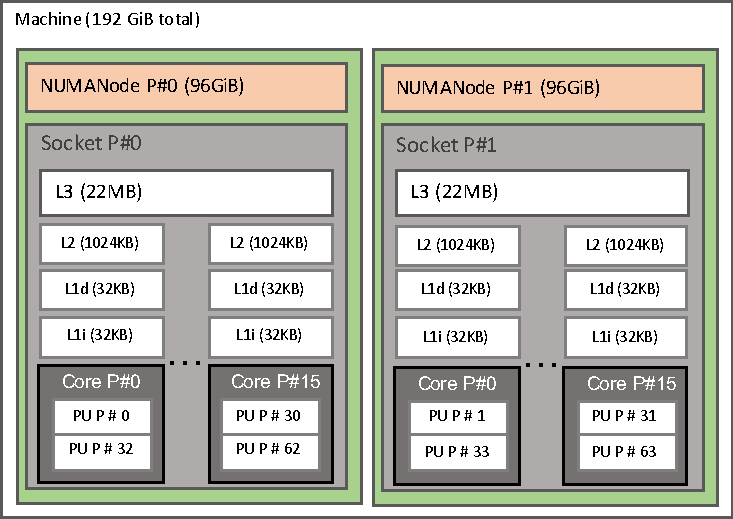
\includegraphics[width=.9\linewidth]{imgs/lstopo}}
    \caption{Topology of the nodes of the cluster \textsf{Dahu}}\label{fig:topo}
\end{figure}
% The advantage of using G5K is having an access to a wide set of physical nodes with different capabilities. 
% The usage procedure is to book a machine for period of time with the chosen OS in less than 5 minutes, ship and run the test script, then release the machine. When a machine is released everything is discarded even the OS.

\subsection{Systems Benchmarks}
Our first criterion to choose the systems benchmarks was the scalability, as we need to run tests at different workloads by choosing the right number of used PU.
The other criteria are the documentation, the accuracy and the references to the benchmark.
\emph{NAS Parallel Benchmark} (NPB v3.3.1)~\cite{Bailey:1991:NPB:125826.125925} is one of the most used suite of benchmarks in the HPC literature and it fulfills our benchmarking requirements.
We mainly used the pseudo application \emph{Lower-Upper symmetric Gauss-Seidel} (\textsf{LU}), the \emph{Conjugate Gradient} (\textsf{CG}) and \emph{Embarrassingly Parallel} (\textsf{EP}) computation-intensive benchmarks in our experiments, with the \textsf{C} data class.
These are the main benchmarks used in many similar works, such as~\cite{heinrich_predicting}.
Nonetheless, in order to validate our results on a wider set of benchmarks and applications, we also used \texttt{Stress-ng v0.10.0},\footnote{\url{https://kernel.ubuntu.com/~cking/stress-ng}} \texttt{pbzip2 v1.1.9},\footnote{\url{https://launchpad.net/pbzip2/}} \texttt{linpack}\footnote{\url{http://www.netlib.org/linpack}} and \texttt{sha256 v8.26}\footnote{\url{https://linux.die.net/man/1/sha256sum}} as representative systems benchmarks to conduct our experiments with a broad diversity of workloads.



\subsection{Measurement Tools \& Methodology}
To study the energy consumption of nodes, we considered Intel \emph{Running Average Power Limit} (RAPL)~\cite{Khan:2018:RAE:3199681.3177754}, which is one of the most accurate tools to report the CPU/DRAM global energy consumption.
We also used \textsc{PowerAPI}~\cite{DBLP:journals/jss/ColmantRKSFS18}, which is a power monitoring toolkit that builds a model over RAPL to compute the energy consumption at process-level when we needed to isolate energy consumption of a single process.
Our clusters are provisioned with a minimal version of Debian\,9 (4.9.0 kernel version) where we install Docker (version 18.09.5), which will be used to run the RAPL sensor and the benchmark itself.
The energy sensor collects RAPL reports and stores them in a remote \textsc{MongoDB} instance, allowing us to perform \emph{post-mortem} analysis in a dedicated environment.
Using Docker makes the deployment process easier on the one hand, and provides us with a built-in control group encapsulation of the conducted tests on the other hand.
This allows \textsc{PowerAPI} to measures all the running containers, even the RAPL sensor consumption, as it is isolated in a container.
One potential threat covers the impact of Docker on the energy variation.
We therefore conducted a preliminary experiment by running the same benchmarks \textsf{LU}, \textsf{CG} and \textsf{EP} in a Docker container and a flat binary format on 3 nodes of the cluster \textsf{Dahu} to assess if Docker induces an additional variation.
Figure~\ref{fig:docker} reports that this is not the case, as the energy consumption variation does not get noticeably affected by Docker while running a same compiled version of the benchmarks at 5\,\%, 50\,\% and 100\,\% workloads.
In fact, while Docker increases the energy consumption due to the extra layer it implements~\cite{eddie_antonio_santos_how}, it does not noticeably affect the energy variation.
The \emph{standard deviation} (STD) is even slightly smaller ($STD_{Docker}=192 mJ$,$STD_{Binary}=207 mJ$), taking into account the measurements errors and the OS activity.

\begin{figure}
    \center{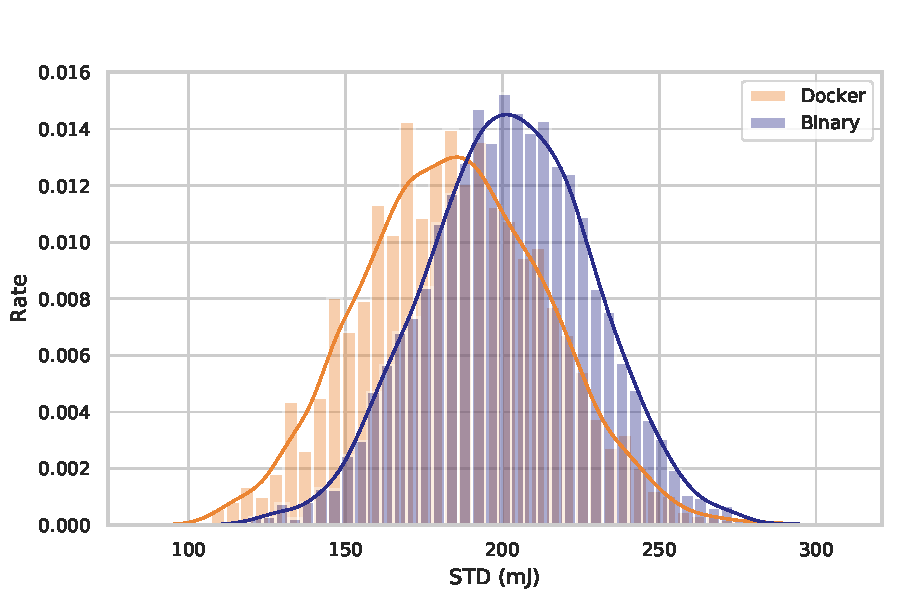
\includegraphics[width=.9\linewidth]{imgs/docvsbin}}
    \caption{Comparing the variation of binary and Docker versions of aggregated \textsf{LU}, \textsf{CG} and \textsf{EP} benchmarks}\label{fig:docker}
\end{figure}

Every experiment is conducted on $100$ iterations, on multiple nodes and using the 3 NPB benchmarks we mentioned, with a warmup phase of 10 iterations for each experiment.
In most cases, we were seeking to evaluate the \emph{STandard Deviation} (STD), which is the most representative factor of the energy variation.
We tried to be very careful, while running our experiments, not to fall in the most common benchmarking "crimes"~\cite{DBLP:journals/corr/abs-1801-02381}.
As we study the STD difference of measurements we observed from empirical experiments, we use the bootstrap method~\cite{efron2000bootstrap} to randomly build multiple subsets of data from the original dataset, and we draw the STD density of those sets, as illustrated in Figure~\ref{fig:docker}.
Given the space constraints, this paper reports on aggregated results for nodes, benchmarks and workloads, but the raw data we collected remains available through the public repository we published.\footnote{\url{https://github.com/anonymous-data/Energy-Variation}}
We believe this can help to achieve better and more reliable comparisons.

We mainly consider 3 different workloads in our experiments: \textsf{single process}, 50\,\%, and 100\,\%, to cover the low, medium and high CPU usage when analyzing the studied parameters effect, respectively.
These workloads reflect the ratio of used PU count to the total available PU.

\section{Energy Variation Analysis}\label{sec:parameters}
In this section, we aim to establish experimental guidelines to reduce the CPU energy variation.
We therefore explore many potential factors and parameters that could have a considerable effect on the energy variation.

\subsection{\textsc{RQ}~1: Benchmarking Protocol}
To achieve a robust and reproducible experiment, practitioners often tend to repeat their tests multiple times, in order to analyze the related performance indicators, such as execution time, memory consumption or energy consumption.
We therefore aim to study the benchmarking protocol to identify how to efficiently iterate the tests to capture a trustable energy consumption evaluation.
% This process of repeating executions should not be random in order to avoid different results because of the CPU behavior, the cache data, the memory size and plenty of other aspects.

In this first experiment, we investigate if changing the testing protocol affects the energy variation.
To achieve this, we considered 3 execution modes:
In the \textsf{"normal"} mode, we iteratively run the benchmark 100 times without any extra command, while the \textsf{"sleep"} mode suspends the execution script for 60\,seconds between iterations.
Finally, the \textsf{"reboot"} mode automatically reboots the machine after each iteration.
The difference between the \textsf{normal} and \textsf{sleep} modes intends to highlight that the CPU needs some rest before starting another iteration, especially for an intense workload.
Putting the CPU into sleep for several seconds could give it some time to reach a lower frequency state or/and reduce its temperature, which could have an impact on the energy variation.
The \textsf{reboot} mode, on the other hand, is the most straightforward way to reset the machine state after every iteration.
It could also be beneficial to reset the CPU frequency and temperature, the stored data, the cache or the CPU registries.
However, the reboot task takes a considerable amount of time, so rebooting the node after every single operation is not the fastest nor the most eco-friendly solution, but it deserves to be checked to investigate if it effectively enhances the overall energy variation or not.

Figure~\ref{fig:running-process} reports on $300$ aggregated executions of the  benchmarks \textsf{LU}, \textsf{CG} and \textsf{EP}, on 4 machines of the cluster \textsf{Dahu} (cf. Table~\ref{table:g5k}) for different workloads.
We note that the results have been executed with different datasets sizes (\textsf{B}, \textsf{C} and \textsf{D} for single process, 50\,\% and 100\,\% respectively) to remedy to the brief execution times at high workloads for small datasets.
This justifies the scale differences of reported energy consumptions between the 3 modes in Figure~\ref{fig:running-process}.
As one can observe, picking one of these strategies does not have a strong impact on the energy variation for most workloads.
In fact, all the strategies seem to exhibit the same variation with all the workloads we considered---\emph{i.e.}, the STD is tightly close between the three modes.
The only exception is the \textsf{reboot} mode at 100\,\% load, where the STD is 150\,\% times worst, due to an important amount of outliers.
This goes against our expectation, even when setting a warm-up time after reboot to stabilize the OS.

\begin{figure*}
    \center{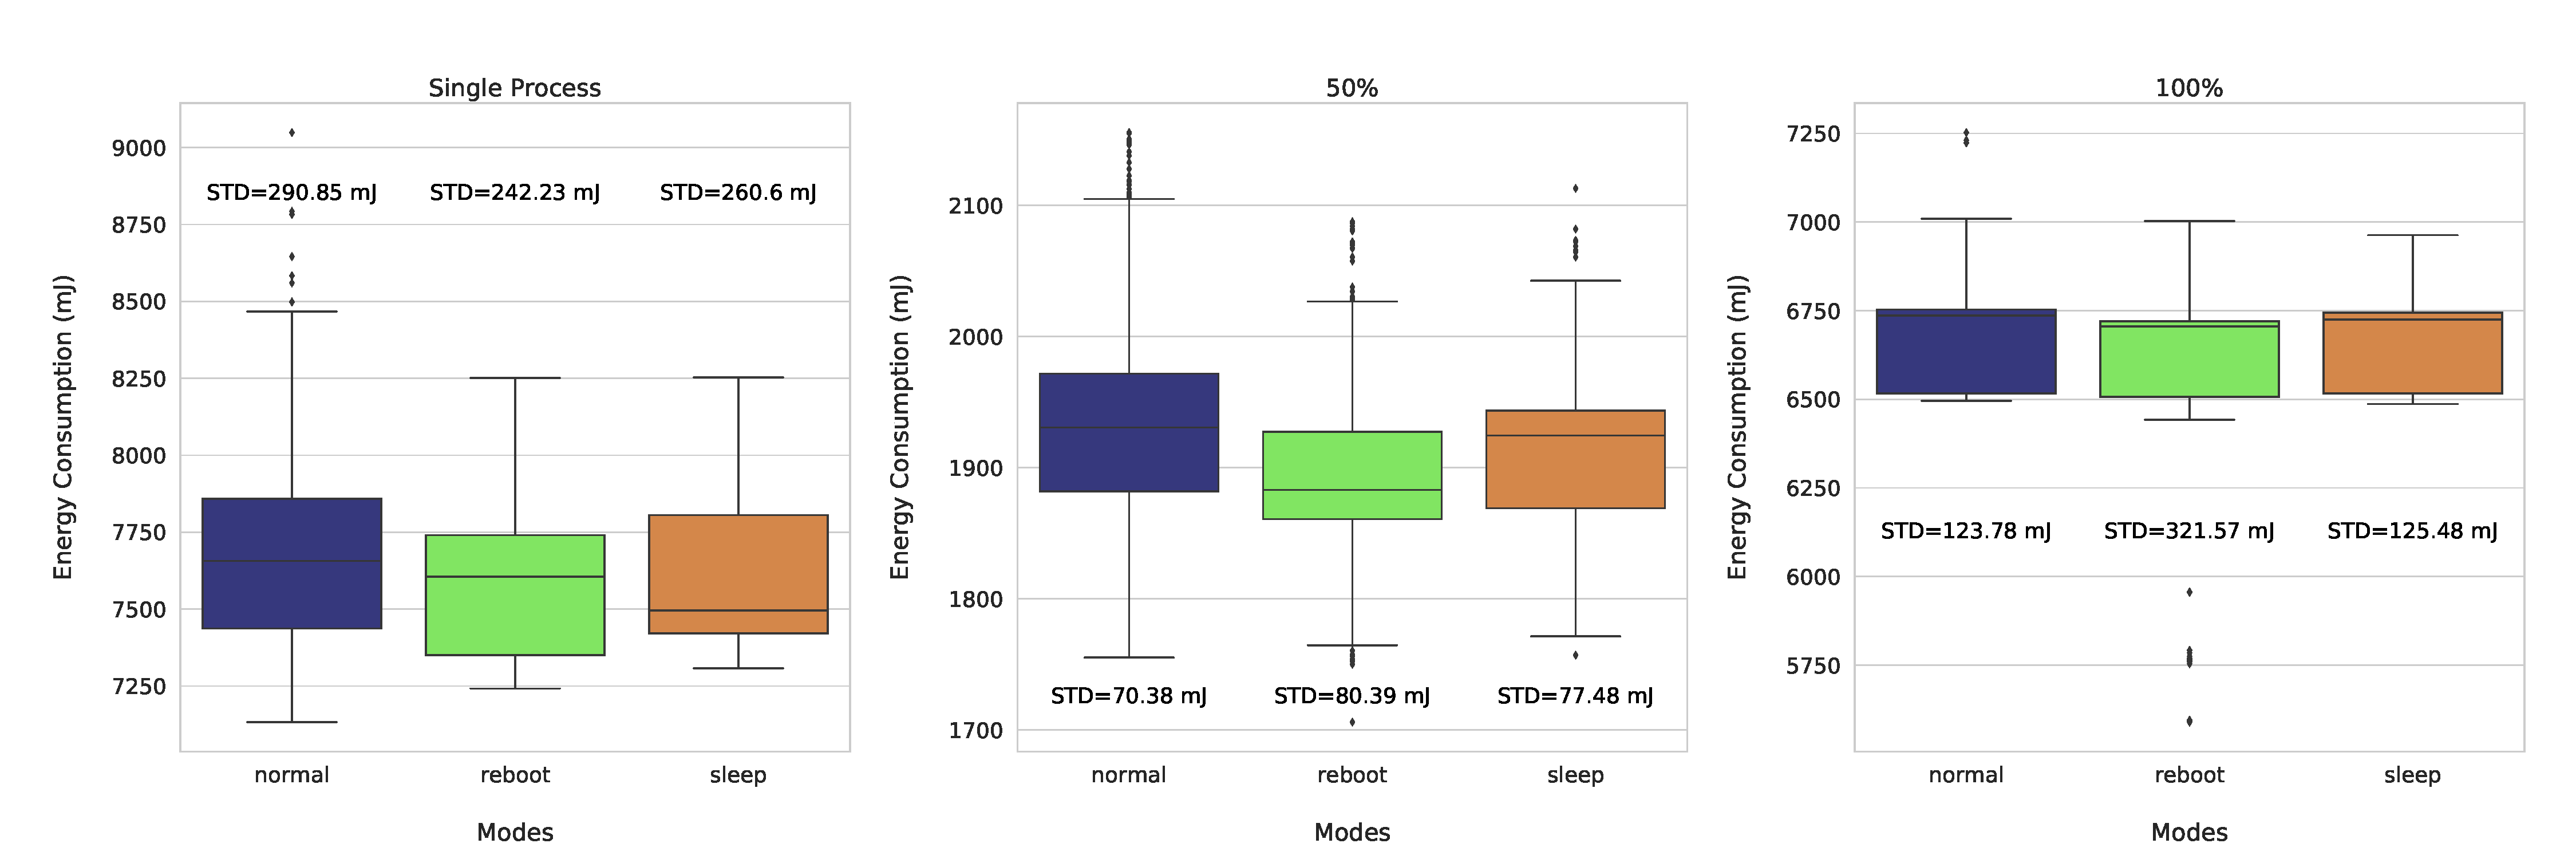
\includegraphics[width=\linewidth]{imgs/running-process}}
    \caption{Energy variation with the \textsf{normal}, \textsf{sleep} and \textsf{reboot} modes}\label{fig:running-process}
\end{figure*}

In Figure~\ref{fig:reboot}, we study the standard deviation of the three modes by constituting $5,000$ random 30-iterations sets from the previous executions set and we compute the STD in each case, considering mainly the 100\,\% workload as the STD was 150\,\% higher for the \textsf{reboot} mode with that load.
We can observe that the considerable amount of outliers in the \textsf{reboot} mode is not negligible, as the STD density is clearly higher than the two other modes.
This makes the \textsf{reboot} mode as the less appropriate for the energy variation at high workloads.

\begin{figure}
    \center{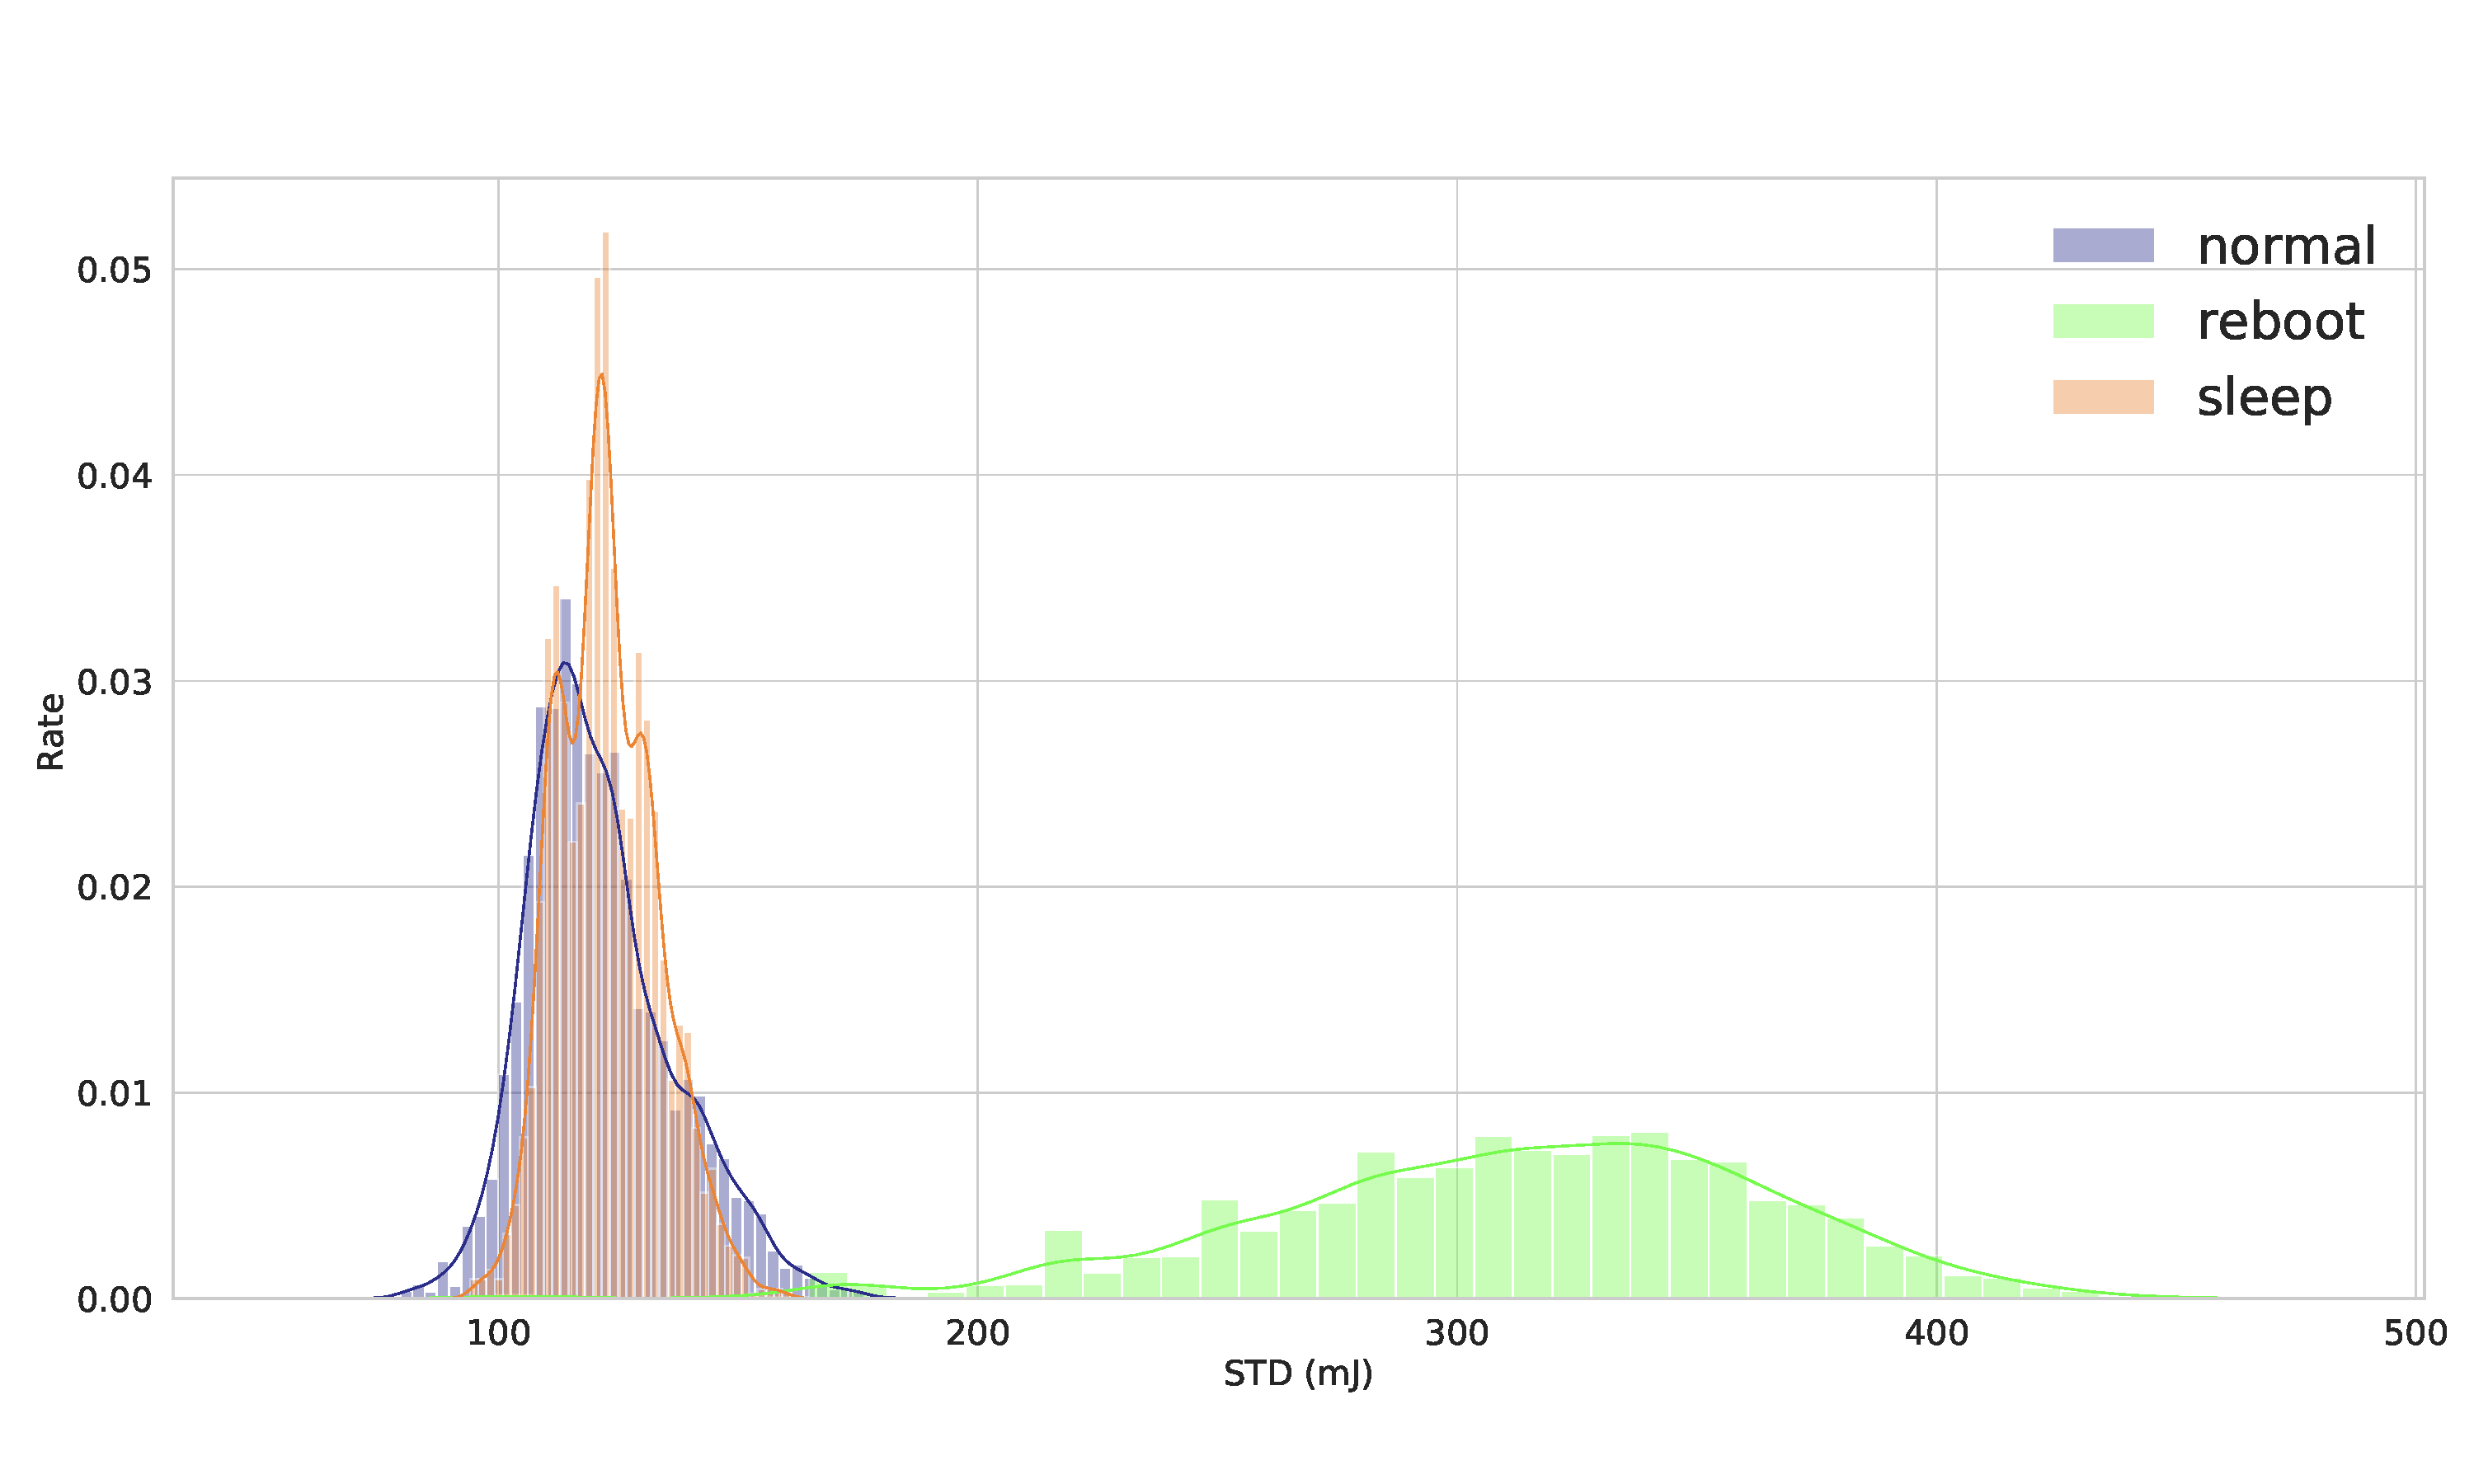
\includegraphics[width=.9\linewidth]{imgs/reboot}}
    \caption{STD analysis of the \textsf{normal}, \textsf{sleep} and \textsf{reboot} modes}\label{fig:reboot}
\end{figure}

\begin{mdframed}[skipabove=\topsep,skipbelow=\topsep]

    To answer \textsc{RQ~1}, we conclude that the benchmarking protocol \textbf{partially affects} the energy variation, as highlighted by the \textsf{reboot} mode results for high workloads.

\end{mdframed}

\subsection{\textsc{RQ}~2: Processor Features}
The C-states provide the ability to switch the CPU between more or less consuming states upon activities.
Turning the C-states on or off have been subject of many discussions~\cite{5463056}, because of its dynamic frequency mechanism but, to the best of our knowledge, there have been no fully conducted C-states behavior analysis on CPU energy variation.

We intend to investigate how much the energy consumption varies when disabling the C-states (thus, keeping the CPU in the \texttt{C0} state) and at which workload.
Figure~\ref{fig:c-states} depicts the results of the experiments we executed on three nodes of the cluster \textsf{Dahu}.
On each node, we ran the same set of benchmarks with two modes: \textsf{C-states on}, which is the default mode, and \textsf{C-states off}.
Each iteration includes 100 executions of the same benchmark at a given workload, with three workload levels.
We note that our results have been confirmed with the benchmarks \texttt{LU}, \texttt{CG} and \texttt{EP}.

We can clearly see the effect that has the \textsf{C-states off} mode when running a single-process application/benchmark.
The energy consumption varies 5~times less than the default mode.
In this case, only one CPU core is used among $2\times16$ physical cores.
The other cores are switched to a low consumption state when C-states are on, the switching operation causes an important energy consumption difference between the cores, and could be affected by other activities, such as the kernel activity, causing a notable energy consumption variation.
On the other hand, switching off the C-states would keep all the cores---even the unused ones---at a high frequency usage.
This highly reduces the variation, but causes up to 50\,\% of extra energy consumption in this test ($Mean_{C-states-off}=11,665 mJ$,$Mean_{C-states-on}=7,641 mJ$).

At a 100\,\% workload, disabling the C-states seems to have no effect on the total energy consumption nor its variation.
In fact, all the cores are used at 100\,\% and the C-states module would have no effect, as the cores are not idle.
The same reason would apply for the 50\,\% load, as the hyper-threading is active on all cores, thus causing the usage of most of them.
For single process workloads, disabling the C-states causes the process to consume 50\,\% more energy as reported in Figure~\ref{fig:c-states}, but reduces the variation by 5~times compared to the \textsf{C-states on} mode.
This leads to mainly two questions: Can a process pinning method reduce/increase the energy variation? And, how does the energy consumption variation evolve at different PU usage level?

\begin{figure*}
    \center{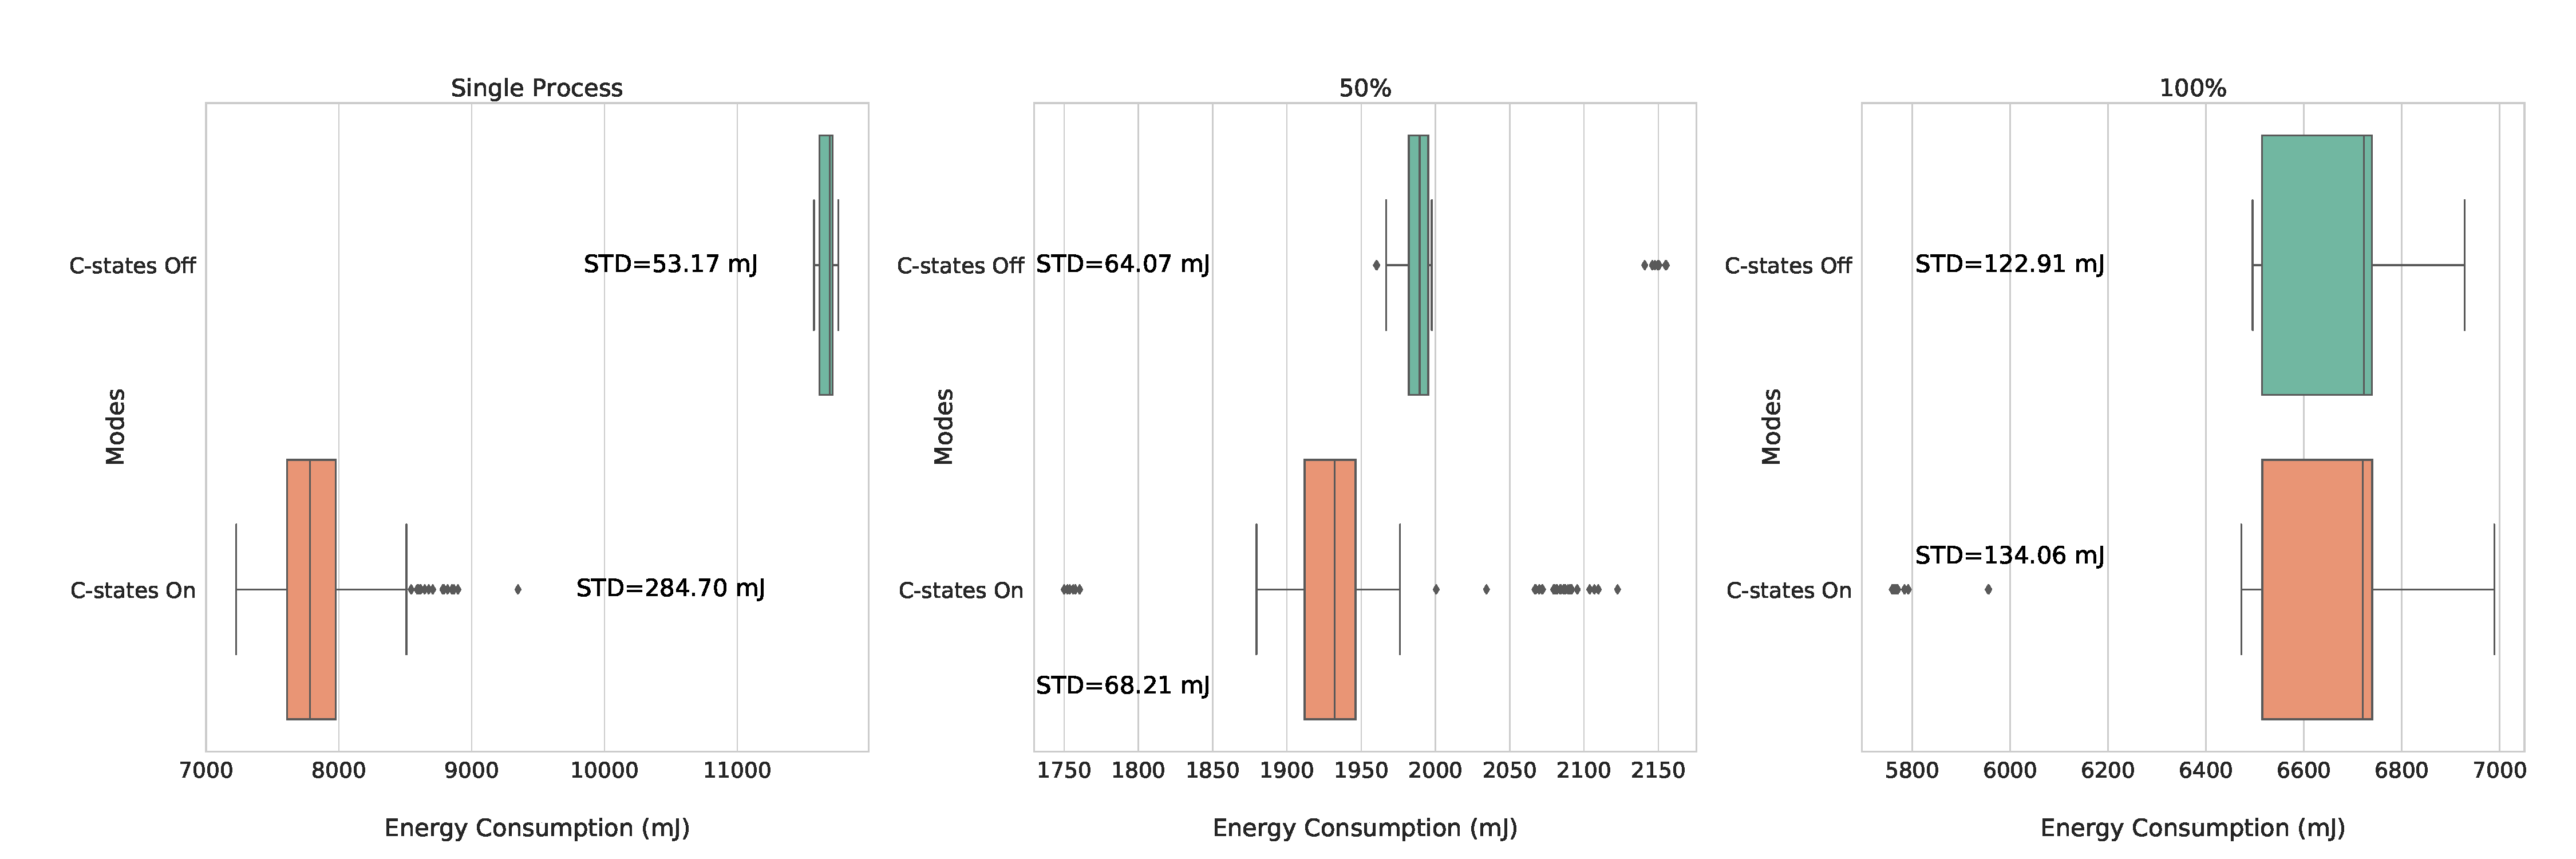
\includegraphics[width=\linewidth]{imgs/c-states}}
    \caption{Energy variation when disabling the C-states}\label{fig:c-states}
\end{figure*}

\subsubsection{Cores Pinning}
To answer the first question, we repeated the previous test at 50\,\% workload.
In this experiment, we considered three cores usage strategies, the first one (\textsf{S1}) would pin the processes on all the PU of one of the two sockets (including hyper-threads), so it will be used at 100\,\%, and leave the other CPU idle.
The second strategy (\textsf{S2}) splits the workload on the two sockets so each CPU will handle 50\,\% of the load.
In this strategy, we only use the core PU and not the hyper-threads PU, so every process would not share his core usage (all the cores are being used).
The third strategy (\textsf{S3}) consists also on splitting the workload between the two sockets, but considering the usage of the hyper-threads on each core---\emph{i.e.}, half of the cores are being used over the two CPU.
Figure~\ref{fig:cores-pinning} reports on the energy consumption of the three strategies when running the benchmark \texttt{CG} on the cluster \textsf{Dahu}.
We can notice the big difference between these three execution modes that we obtained only by changing the PU pinning method (that we acknowledged with more than 100 additional runs over more than 30 machines and with the benchmarks \texttt{LU} and \texttt{EP}).
For example, \textsf{S2} is the least power consuming strategy.
We argue that the reason is related to the isolation of every process on a single physical core, reducing the context switch operations.
In the first and third strategy, $32$ processes are being scheduled on $16$ physical cores using the hyper-threads PU, which will introduce more context switching, and thus more energy consumption.

\begin{figure}
    \center{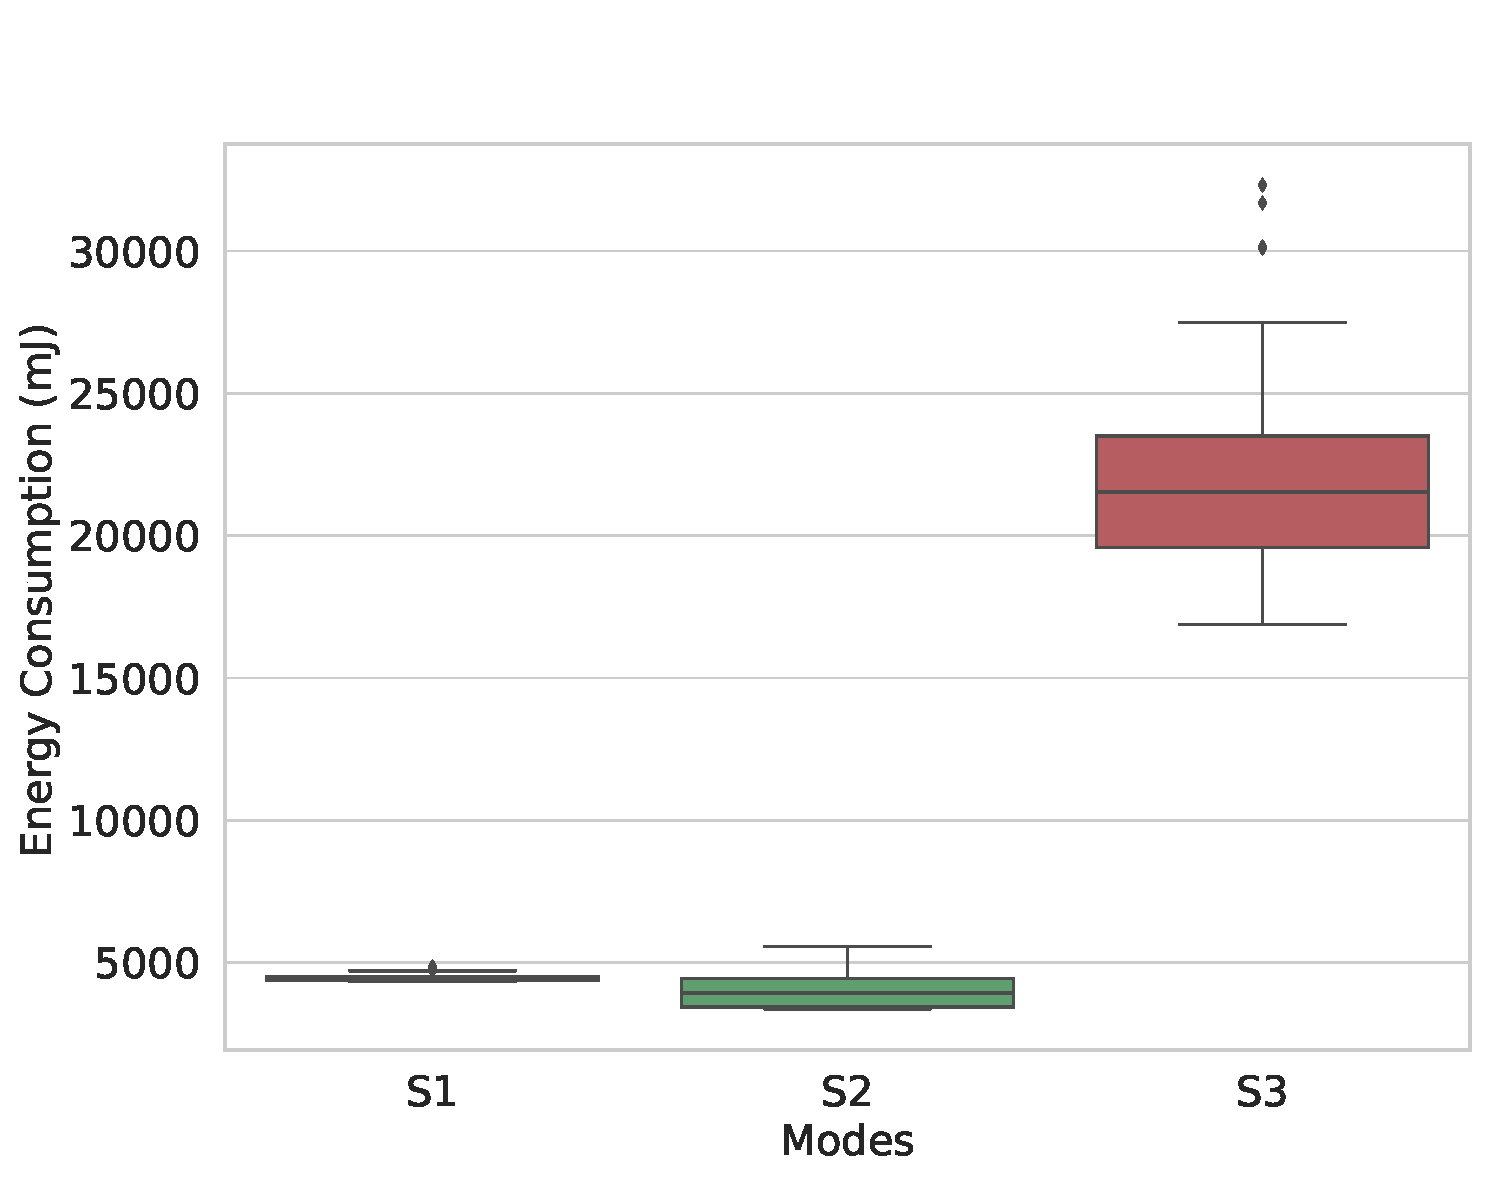
\includegraphics[width=.8\linewidth]{imgs/cores_pinning}}
    \caption{Energy variation considering the three cores pinning strategies at 50\,\% workload}\label{fig:cores-pinning}
\end{figure}

We note that even if the first and third strategies are very similar (both use hyper-threads, but only on one CPU for the first and on two CPU for the third), the gap between them is considerable variation-wise, as the variation is 30 times lower in the first strategy ($STD_{S1}=116 mJ$,$STD_{S3}=3,452 mJ$).
This shows that the usage of the hyper-threads technology is not the main reason behind the variation, the first strategy has even less variation than the second one and still uses the hyper-threading.

The reason for the \textsf{S1} low energy consumption is that one of the two sockets is idle and will likely be in a lower power P-state, even with the disabled C-states.
The \textsf{S2} case is also low energy consuming because by distributing the threads across all the cores, it completes the task faster than in the other cases.
Hence, it consumes less energy.
The \textsf{S3} is a high consuming strategy because both sockets are being used, but only half the cores are active.
This means that we pay the energy cost for both sockets being operational and for the experiments taking longer to run because of the recurrent context switching.

Our hypothesis regarding the worst results that we observed when using the third strategy is the recurrent context switching, added to the OS scheduling that could reschedule processes from a socket to another, which invalids the cache usage as a process can not take profit of the socket local L3 cache when it moves from a CPU to another (cf. Figure~\ref{fig:topo}).

Moreover, the fact that the variation is 4--5 times higher when using the strategy \textsf{S2} compared to \textsf{S1} ($STD_{S1}=116 mJ$, $STD_{S3}=575 mJ$), gives another reason to believe that swapping a process from a CPU to another increases the variation due to CPU micro~differences, cache misses and cache coherency.
While the mean execution time for the strategy \textsf{S3} is very high ($MeanTime_{S3}= 46 s$) compared to the two other strategies ($MeanTime_{S1}= 11 s$, $MeanTime_{S2}= 7 s$), we see no correlation between the execution time and the energy variation, as the \textsf{S1} still give less variations than \textsf{S2} even if it takes 36\,\% more time to run.

Table~\ref{table:corespinning} reports on additional aggregated results for the STD comparison on four other nodes of the cluster \textsf{Dahu} at 50\,\%, with the benchmarks \textsf{LU}, \textsf{CG} and \textsf{EP}.
In fact, the CPU usage strategy \textsf{S1} is by far the experimentation mode that gave the least variation.
The STD is almost 5 times better than the strategy \textsf{S2}, but is up to 10\,\% more energy consuming ($Mean_{S1}=4469 mJ$, $Mean_{S2}=4016 mJ$).
On the other hand, the strategy \textsf{S3} is the worst, where the energy consumption can be up to 5 times higher than the strategy \textsf{S2} ($Mean_{S2}=4016 mJ$, $Mean_{S3}=21645 mJ$) and the variation is much worst (30 times compared to the first strategy).
These results allow us to have a better understanding of the different processes-to-PU pinning strategies, where isolating the workload on a single CPU is the best strategy.
Using the hyper-threads PU on multiple sockets seems to be a bad recommendation, while keeping the hyper-threading enabled on the machine is not problematic, as long as the processes are correctly pinned on the PU.
Our experiments show that running one hyper-thread per core is not always the best to do, at the opposite of the claims of~\cite{marathe_empirical_2017_m}.

\begin{table}
    \centering
    \caption{STD (mJ) comparison for 3 pinning strategies}
    \label{table:corespinning}
    \small
    \begin{tabular}{|l|l|l|l|}
        \hline
        \textbf{Strategy} & \textbf{S1} & \textbf{S2} & \textbf{S3} \\
        \hline
        \hline
        \textbf{Node~1}   & 88          & 270         & 1,654       \\
        \hline
        \textbf{Node~2}   & 79          & 283         & 2,096       \\
        \hline
        \textbf{Node~3}   & 58          & 287         & 1,725       \\
        \hline
        \textbf{Node~4}   & 51          & 229         & 1,334       \\
        \hline
    \end{tabular}
\end{table}

\subsubsection{Processes Threshold}
To answer the second question regarding the evolution of the energy variation at different levels of CPU usage, we varied the used PU's count to track the EV evolution.
Figure~\ref{fig:process-tresh} compares the aggregated energy variation when the C-states are on and off using 2, 4 and 8 processes for the benchmarks \textsf{LU}, \textsf{CG} and \textsf{EP}.
This figure confirms that disabling the CPU C-states does not decrease the variation for all the workloads, as we can clearly observe, the variation is increasing along with the number of processes.
When running only 2 processes, turning off the C-states reduces the STD up to 6~times, but consumes 20\,\% more energy ($Mean_{C-states-on}=10,334 mJ$, $Mean_{C-states-off}=12,594 mJ$).
This variation is 4~times lower when running 4 processes and almost equal to the \textsf{C-states on} mode when running 8 processes.
In fact, running more processes implies to use more CPU cores, which reduces the idle cores count, so the cores will more likely stay at a higher consumption state even if the C-states mechanism is on.

In our case, using 4 PU reduces the variation by 4~times and consumes almost the same energy as keeping the C-states mechanism on ($Mean_{C-states-on}=7,048 mJ$, $Mean_{C-states-off}=7,119 mJ$).
This case would be the closest to reality as we do not want to increase the energy consumption while reducing the variation, but using a lower number of PU still results in less variation, even if it increases the overall energy consumption.

\begin{figure*}
    \center{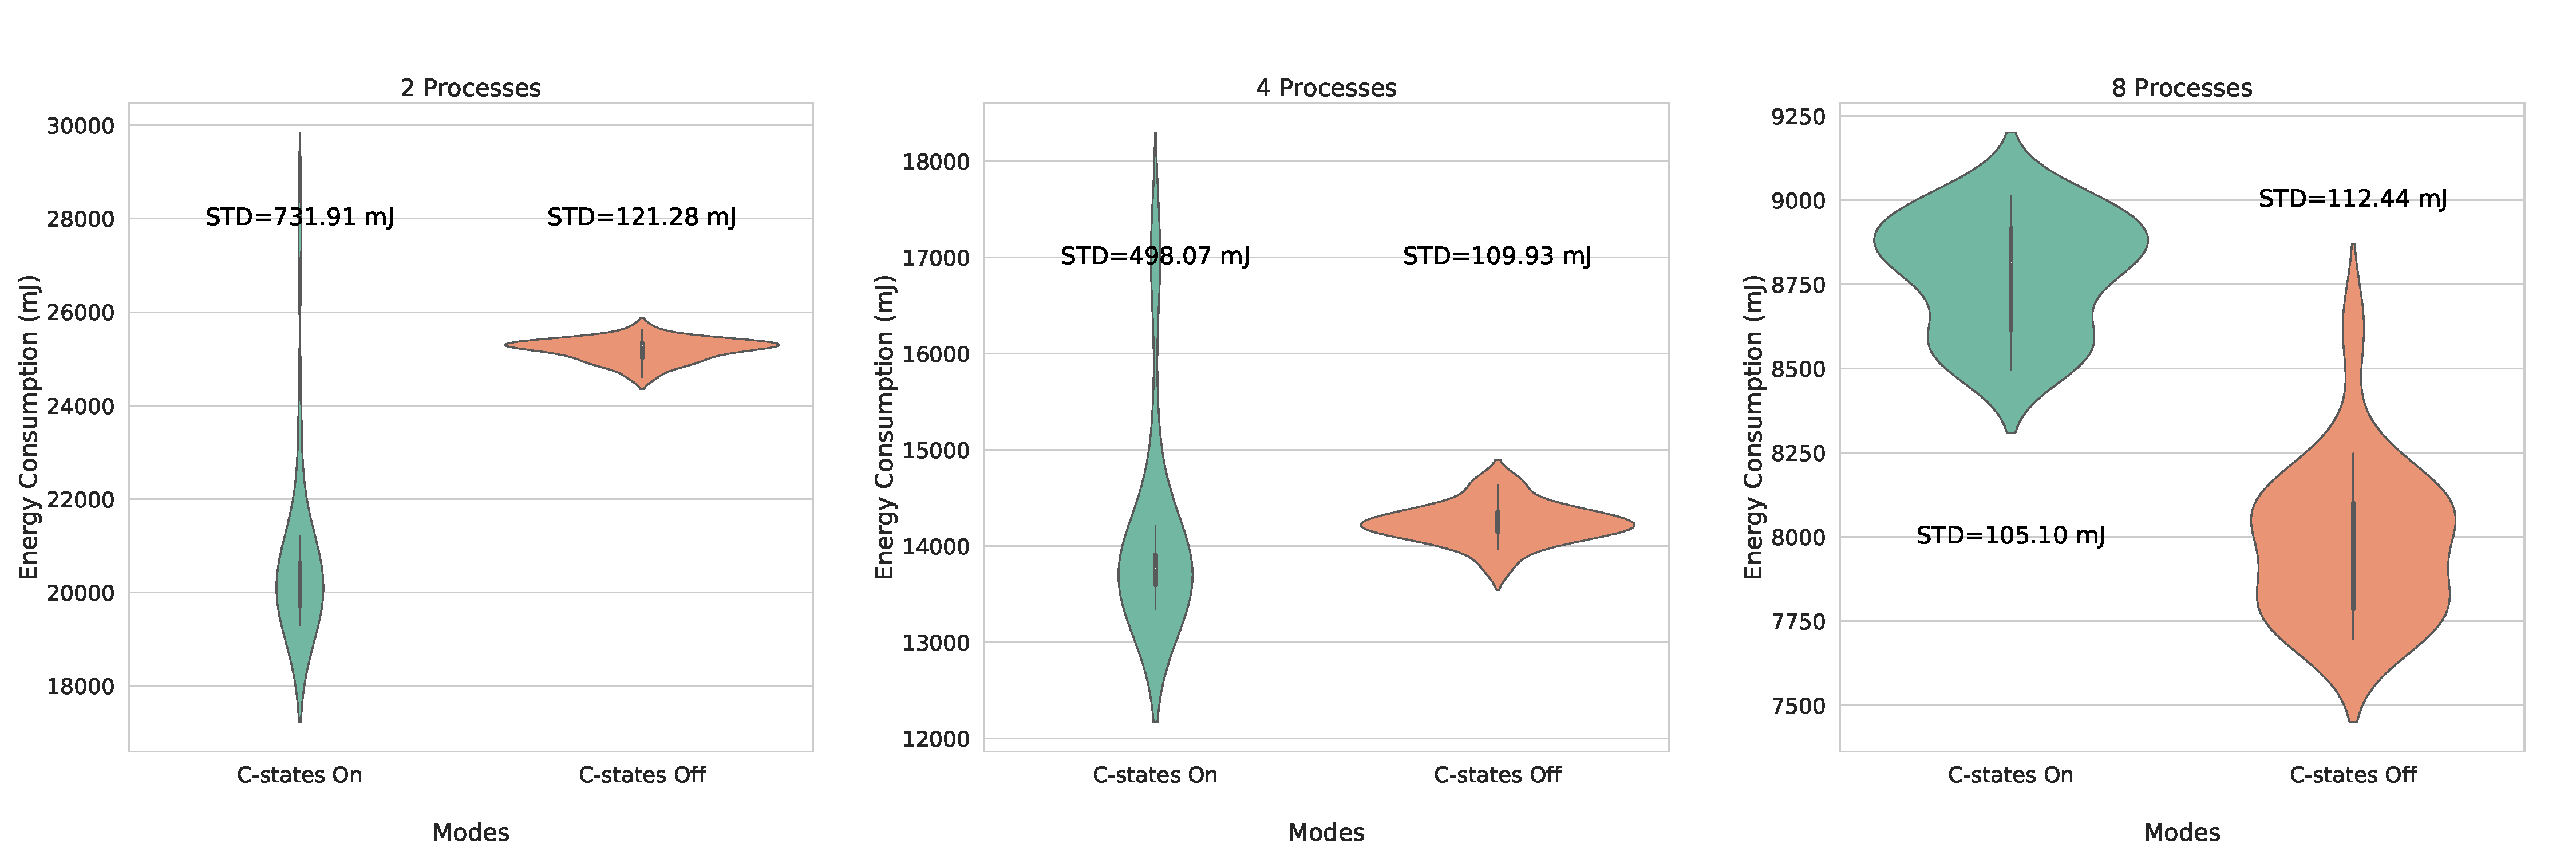
\includegraphics[width=\linewidth]{imgs/tresh}}
    \caption{C-states effect on the energy variation, regarding the application processes count}\label{fig:process-tresh}
\end{figure*}

We note that disabling the C-states is not recommended in production environments, as it introduces extra energy consumption for low workloads (around 50\,\% in our case for a single process job).
However, our goal is not to optimize the energy consumption, but to minimize the energy variation.
Thus, disabling the C-states is very important to stabilize the measurements in some cases when the variation matters the most.
Comparing the energy consumptions of two algorithms or two versions of a software systems is an example of use case benefiting from this recommendation.

\subsubsection{Turbo Boost}
The Turbo Boost---also known as \emph{Dynamic Overclocking}---is a feature that has been incorporated in Intel CPU since the Sandy~Bridge micro-architecture, and is now widely available on all of the Core\,i5, Core\,i7, Core\,i9 and Xeon series.
It automatically raises some of the CPU cores operating frequency for short periods of time, and thus boost performances under specific constraints.
When demanding tasks are running, the operating system decides on using the highest performance state of the processor.

Disabling or enabling the Turbo~Boost has a direct impact on the CPU frequency behavior, as enabling it allows the CPU to reach higher frequencies in order to execute some tasks for a short period of time.
However, its usage does not have a trivial impact on the energy variation.
Acun~\emph{et~al.}~\cite{acun_variation_2016} tried to track the Turbo~Boost impact on the Ivy~Bridge and the Sandy~Bridge architectures.
They concluded that it is one of the main responsible for the energy variation, as it increases the variation from 1\,\% to 16\,\%.
In our study, we included a Turbo~Boost experiment in our testbed, to check this property on the recent Xeon Gold processors, covering various workloads.

The experiment we conducted showed that disabling the Turbo Boost does not exhibit any considerable positive or negative effect on the energy variation.
Table~\ref{table:turboboost} compares the STD when enabling/disabling the Turbo~Boost, where the columns are a combination of workload and benchmark.
In fact, we only got some minor measurements differences when switching on and off the Turbo~Boost, and where in favor or against the usage of the Turbo~Boost while repeating tests, considering multiple nodes and benchmarks.
This behavior is mainly related to the \emph{thermal design power} (TDP), especially at high workloads executions.
When a CPU is used at its maximum capacity, the cores would be heating up very fast and would hit the maximum TDP limit.
In this case, the Turbo~Boost cannot offer more power to the CPU because of the CPU thermal restrictions.
At lower workloads, the tests we conducted proved that the Turbo~Boost is not one of the main reasons of the energy variation.
In fact, the variation difference is barely noticeable when disabling the Turbo~Boost, which cannot be considered as a result regarding the OS activity and the measurement error margin.
We cannot affirm that the Turbo~Boost does not have an impact on all the CPU, as we only tested on two recent Xeon CPU (clusters \textsf{Chetemi} and \textsf{Dahu}).
We confirmed our experiments on these machines 100 times at 5\,\%, 25\,\%, 50\,\% and 100\,\% workloads.

\begin{table}%[h!]
    \centering
    \caption{STD (mJ) comparison when enabling/disabling the Turbo~Boost}
    \label{table:turboboost}
    \small
    \begin{tabular}{|c|r|r|}
        \hline
        \textbf{Turbo Boost}  & \textbf{Enabled} & \textbf{Disabled} \\
        \hline
        \hline
        \textsf{EP} / 5\,\%   & 310              & 308               \\
        \hline
        \textsf{CG} / 25\,\%  & 95               & 140               \\
        \hline
        \textsf{LU} / 25\,\%  & 204              & 240               \\
        \hline
        \textsf{EP} / 50\,\%  & 84               & 79                \\
        \hline
        \textsf{EP} / 100\,\% & 125              & 110               \\
        \hline
    \end{tabular}
\end{table}


\begin{mdframed}[skipabove=\topsep,skipbelow=\topsep]
    We conclude that CPU features \textbf{highly impact} the energy variation as an answer for \textsc{RQ~2}.
\end{mdframed}

\subsection{\textsc{RQ}~3: Operating System}
The \emph{operating system} (OS) is the layer that exploits the hardware capabilities efficiently.
It has been designed to ease the execution of most tasks with multitasking and resource sharing.
In some delicate tests and measurements, the OS activity and processes can cause a significant overhead and therefore a potential threat to the validity. % experiments validity
The purpose behind this experiment is to determine if the sampled consumption can be reliably related to the tested application, especially for low-workload applications where CPU resources are not heavily used by the application.

The first way to do is to evaluate the OS idle activity consumption, and to compare it to a low workload running job.
Therefore, we ran 100 iterations of a single process benchmark \textsf{EP}, \textsf{LU} and \textsf{CG} on multiple nodes from the cluster \textsf{Dahu}, and compared the energy behavior of the node with its idle state on the same duration.
The aggregated results, illustrated in Figure~\ref{fig:os-idle}, depict that the idle energy variation is up to 140\,\% worst than when running a job, even if it consumes 120\,\% less energy ($Mean_{Job}=8,746 mJ$, $Mean_{Idle}=3,927 mJ$).
In fact, for the three nodes, randomly picked from the cluster \textsf{Dahu}, the idle variation is way more important than when a test was running, even if it is a single process test on a $32$-cores node.
This result shows that OS idle consumption varies widely, due to the lack of activity and the different CPU frequencies states, but it does not mean that this variation is the main responsible for the overall energy variation.
The OS behaves differently when a job is running, even if the amount of available cores is more than enough for the OS to keep his idle behavior when running a single process.

\begin{figure}
    \center{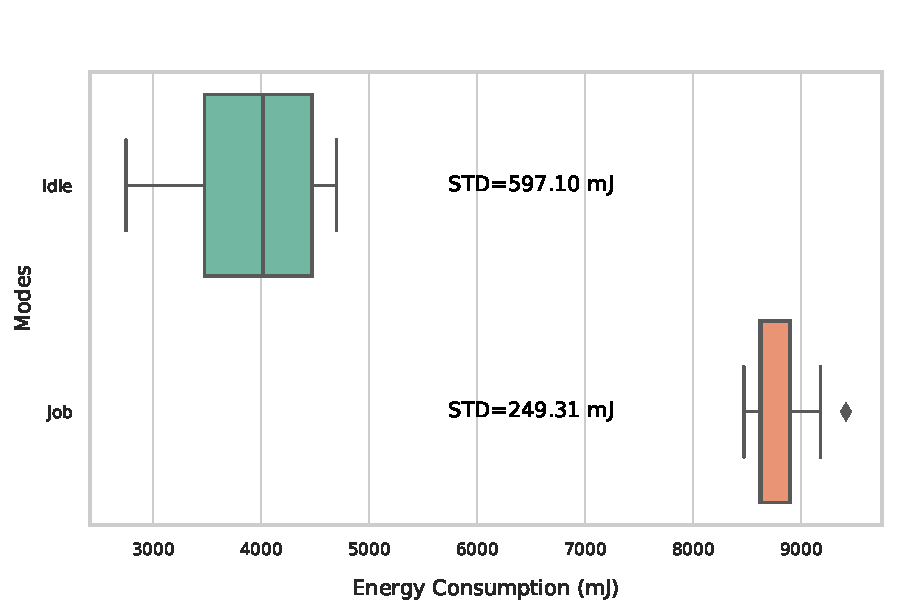
\includegraphics[width=.9\linewidth]{imgs/idle}}
    \caption{OS consumption between idle and when running a single process job}\label{fig:os-idle}
\end{figure}

Inspecting the OS idle energy variation is not sufficient to relate the energy variation to the active job.
In fact, the OS can behave differently regarding the resource usage when running a task.
To evaluate the OS and the job energy consumption separately, we used the \textsc{PowerAPI} toolkit.
This fine-grained power~meter allows the distribution of the RAPL global energy across all the Cgroups of the OS using a power model.
Thus, it is possible to isolate the job energy consumption instead of the global energy consumption delivered by RAPL.
To do so, we ran tests with a single process workload on the cluster \textsf{Dahu}, and used the \textsc{PowerAPI} toolkit to measure the energy consumption.
Then, we compared the job energy consumption to the global RAPL data.
We calculated the Pearson correlation~\cite{ref1} of the energy consumption and variation between global RAPL and \textsc{PowerAPI}, as illustrated in Figure~\ref{fig:correlation}.
The job energy consumption and variation are strongly correlated with the global energy consumption and variation with the coefficients 93.6\,\% and 85.3\,\%, respectively.
However, this does not completely exclude the OS activity, especially if the jobs have tight interaction with the OS through the signals and system calls.
This brings a new question on whether applying extra-tuning on a minimal OS would reduce the variation? As well as what is the effect of the Meltdown security patch---that is known to be causing some performance degradation~\cite{Kocher2018spectre,Lipp2018meltdown}---on the energy variation?

\begin{figure}
    \center{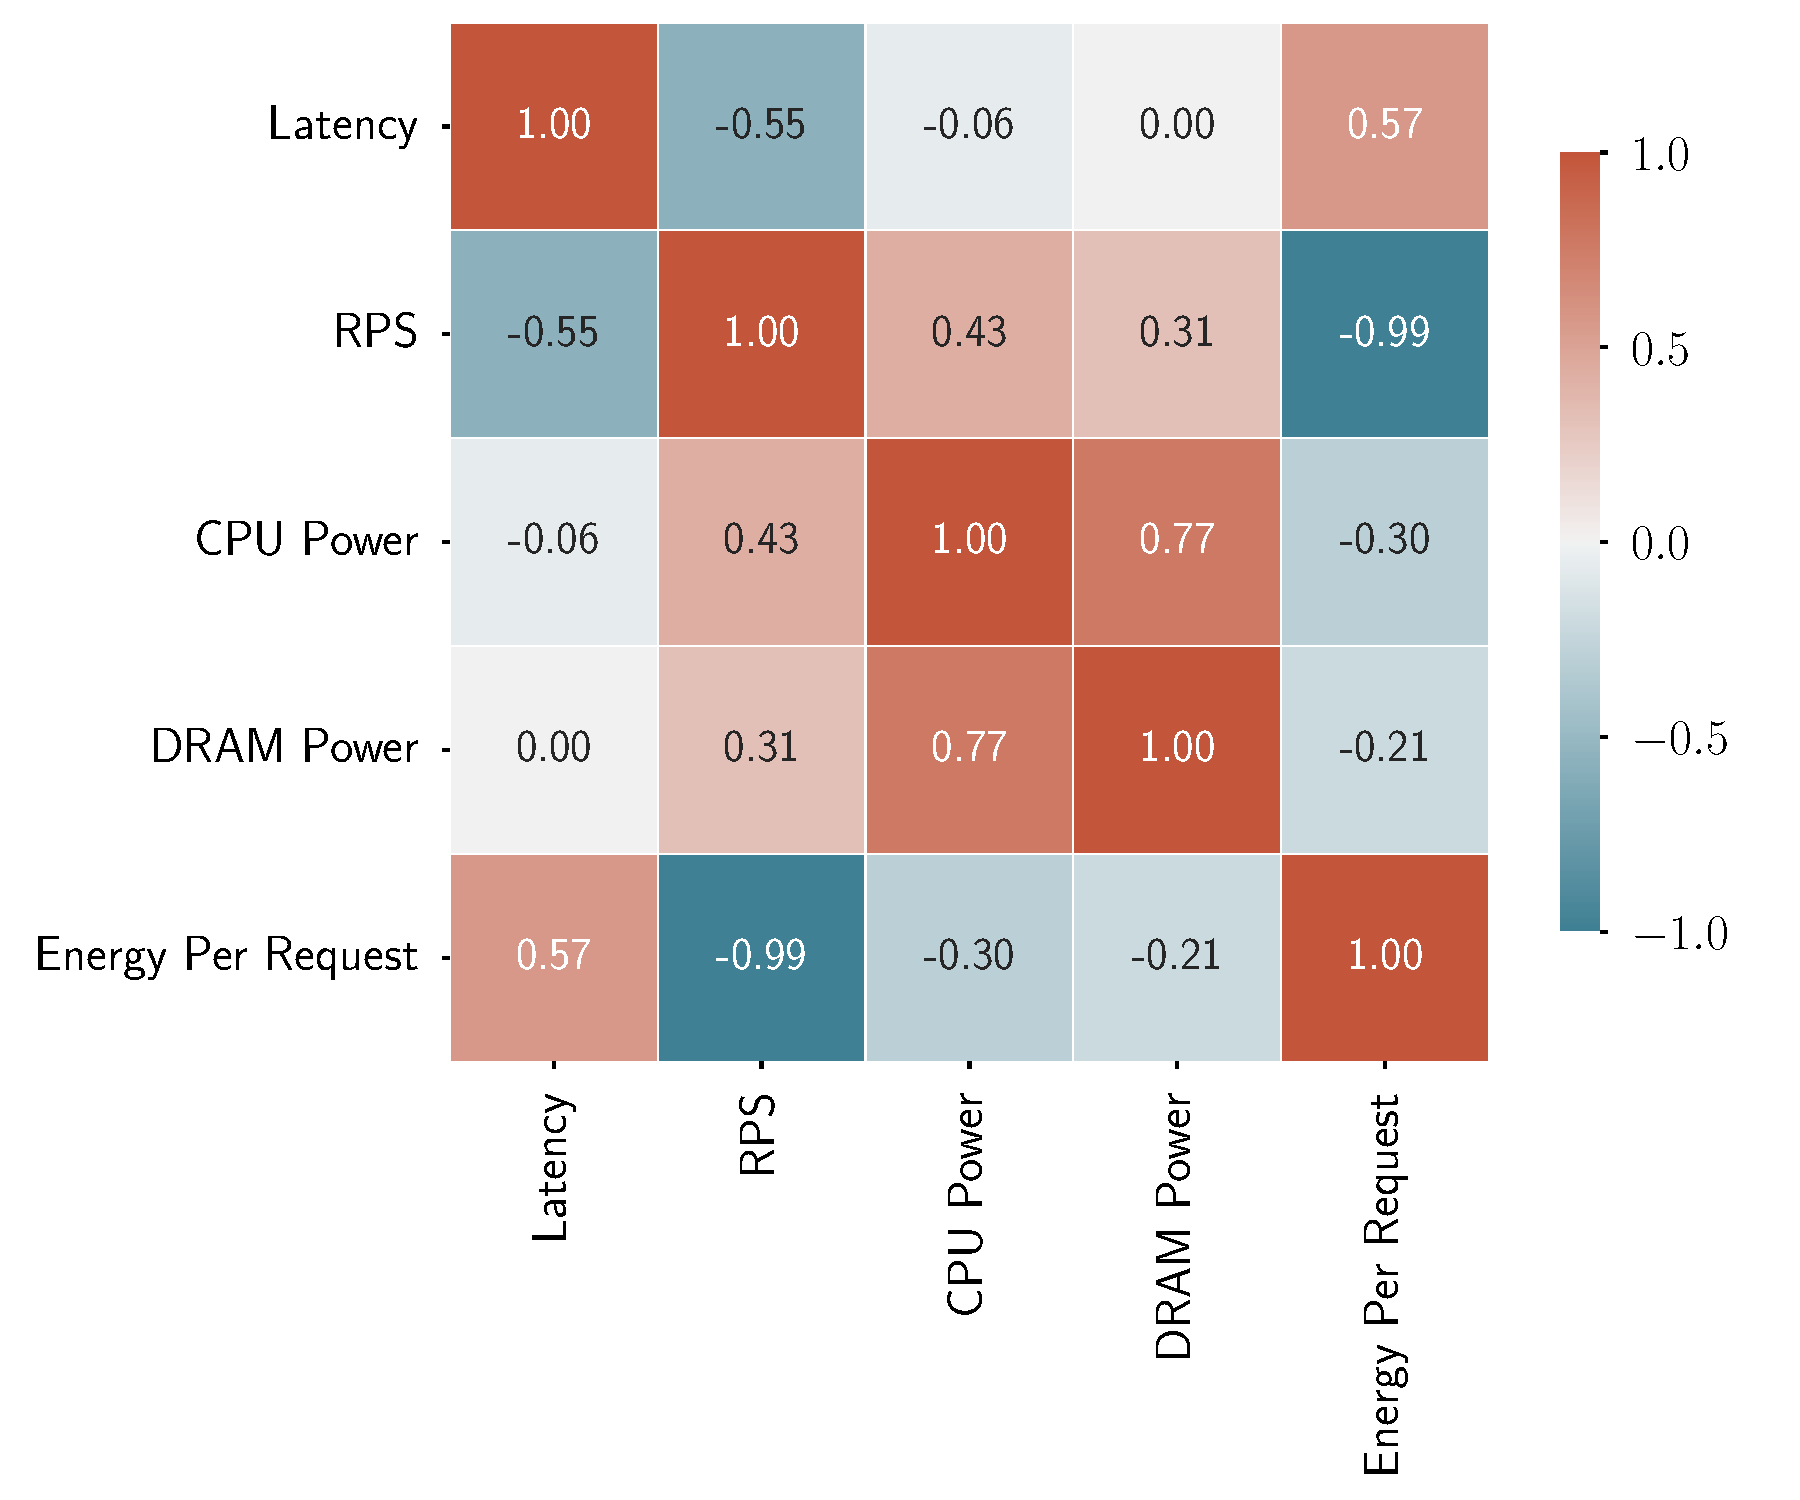
\includegraphics[width=.8\linewidth]{imgs/correlation}}
    \caption{The correlation between the RAPL and the job consumption and variation}\label{fig:correlation}
\end{figure}

\subsubsection{OS Tuning}
An OS is a pack of running processes and services that might or not be required its execution.
In fact, even using a minimal version of a Debian Linux, we could list many OS running services and process that could be disabled/stopped without impacting the test execution.
This extra-tuning may not be the same depending on the nature of the test or the OS.
Thus, we conducted a test with a deeply-tuned OS version.
We disabled all the services/processes that are not essential to the OS/test running, including the OS networking interfaces and logging modules, and we only kept the strict minimum required to the experiment's execution.
Table~\ref{table:osmin} reports on the aggregated results for running single process measurements with the benchmarks \textsf{CG}, \textsf{LU} and \textsf{EP}, on three servers of the cluster \textsf{Dahu}, before and after tuning the OS.
Every cell contains the \emph{STD} value before the tuning, plus/minus a ratio of the energy variation after the tuning.
We notice that the energy variation varies less than 10\,\% after the extra-tuning.
We argue that this variation is not substantial, as it is not stable from a node to another.
Moreover, 10\,\% of variation is not a representative difference, due to many factors that can affect it as the CPU temperature or the measurement errors.

\begin{table}
    \centering
    \caption{STD (mJ) comparison before/after tuning the OS}
    \label{table:osmin}
    \small
    \begin{tabular}{|c|c|c|c|}
        \hline
        \textbf{Node} & \textbf{\sf EP} & \textbf{\sf CG} & \textbf{\sf LU} \\
        \hline
        \hline
        \textbf{N1}   & 1370~-9\,\%     & 78~+7\,\%       & 128~+2\,\%      \\
        \hline
        \textbf{N2}   & 1278~-7\,\%     & 64~-1\,\%       & 120~+9\,\%      \\
        \hline
        \textbf{N3}   & 1118~+1\,\%     & 83~+2\,\%       & 93~+7\,\%       \\
        \hline
    \end{tabular}
\end{table}
% \subsubsection{Meltdown Security Patch}

\subsubsection{Speculative Executions}
Meltdown and Spectre are two of the most famous hardware vulnerabilities discovered in 2018, and exploiting them allows a malicious process to access others processes data that is supposed to be private~\cite{Kocher2018spectre,Lipp2018meltdown}.
They both exploit the speculative execution technique where a process anticipates some upcoming tasks, which are not guaranteed to be executed, when extra resources are available, and revert those changes if not.
Some OS-level patches had been applied to prevent/reduce the criticality of these vulnerabilities.
On the Linux kernel, the patch has been automatically applied since the version 4.14.12.
It mitigates the risk by isolating the kernel and the user space and preventing the mapping of most of the kernel memory in the user space.
% These patches have been reported as decreasing the performance of a system. 
Nikolay~\emph{et~al.} have studied in~\cite{DBLP:journals/corr/abs-1801-04329} the impact of patching the OS on the performance.
The results showed that the overall performance decrease is around 2--3\,\% for most of the benchmarks and real-world applications, only some specific functions can meet a high performance decrease.
In our study, we are interested in the applied patch's impact on the energy variation, as the performance decrease could mean an energy consumption increase.
Thus, we ran the same benchmarks \textsf{LU}, \textsf{CG} ad \textsf{EP} on the cluster \textsf{Dahu} with different workloads, using the same OS, with and without the security patch.
Table~\ref{table:meltdown} reports on the STD values before disabling the security patch.
A minus means that the energy varies less without the patch being applied, while a plus means that it varies more.
These results help us to conclude that the security patch's effect on the energy variation is not substantial and can be absorbed through the error margin for the tested benchmarks.
In fact, the best case to consider is the benchmark \textsf{LU} where the energy variation is less than 10\,\% when we disable the security patch, but this difference is still moderate.
The little performance difference discussed in~\cite{Kocher2018spectre,Lipp2018meltdown} may only be responsible of a small variation, which will be absorbed through the measurement tools and external noise error margin in most cases.

\begin{table}[h!]
    \centering
    \caption{STD (mJ) comparison with/without the security patch}
    \label{table:meltdown}
    \small
    \begin{tabular}{|l|c|c|c|}
        \hline
        \textbf{Node} & \textbf{\sf EP} & \textbf{\sf CG} & \textbf{\sf LU} \\
        \hline
        \hline
        \textbf{N1}   & 269~+2\,\%      & 83~+1\,\%       & 108~-6\,\%      \\
        \hline
        \textbf{N2}   & 195~+1\,\%      & 84~-5\,\%       & 121~-9\,\%      \\
        \hline
        \textbf{N3}   & 223~+/-1\,\%    & 72~-4\,\%       & 117~+8\,\%      \\
        \hline
        \textbf{N4}   & 276~+3\,\%      & 60~+0\,\%       & 113~-3\,\%      \\
        \hline
    \end{tabular}
\end{table}

\begin{mdframed}[skipabove=\topsep,skipbelow=\topsep]
    To answer \textsc{RQ~3}, we conclude that the OS \textbf{should not be the main focus} of the energy variation taming efforts.
\end{mdframed}

\subsection{\textsc{RQ}~4: Processor Generation}
Intel microprocessors have noticeably evolved during these last 20 years.
Most of the new CPU come with new enhancements to the chip density, the maximum Frequency or some optimization features like the C-states or the Turbo~Boost.
This active evolution caused that different generations of CPU can handle a task differently.
The aim of this expriment is not to justify the evolution of the variation across CPU versions/generations, but to observe if the user can choose the best node to execute her experiments.
Previous papers have discussed the evolution of the energy consumption variation across CPU generations and concluded that the variation is getting higher with the latest CPU generations~\cite{wang_experimental_nodate,marathe_empirical_2017_m}, which makes measurements stability even worse.
In this experiment, we therefore compare four different generations of CPU with the aim to evaluate the energy variation for each CPU and its correlation with the generation.
Table~\ref{table:cpus} indicates the characteristics of each of the tested CPU.

\begin{table}
    \centering
    \caption{STD (mJ) comparison of experiments from 4 clusters}
    \small
    \begin{tabular}{|l|c|c|c|c|}
        \hline
        \textbf{Cluster} & \textbf{Dahu} & \textbf{Chetemi} & \textbf{Ecotype} & \textbf{Paranoia} \\
        \hline
        \hline
        Arch             & Skylake       & Broadwell        & Broadwell        & Ivy Bridge        \\
        \hline
        Freq             & 3.7\,GHz      & 3.1\,GHz         & 2.9\,GHz         & 3.0\,GHz          \\
        \hline
        TDP              & 125 W         & 85 W             & 55 W             & 95 W              \\
        \hline
        \hline
        5\%              & 364           & 210              & \textbf{75}      & \textbf{76}       \\
        \hline
        50\%             & 98            & 86               & \textbf{49}      & 244               \\
        \hline
        100\%            & 119           & 116              & \textbf{106}     & 240               \\
        \hline
    \end{tabular}
    \label{table:cpus}
\end{table}

Table~\ref{table:cpus} also shows the aggregated energy variation of the different generations of nodes for the benchmarks \textsf{LU}, \textsf{CG} and \textsf{EP}.
The results attest that the latest versions of CPU do not necessarily cause more variation.
In the experiments we ran, the nodes from the cluster \textsf{Paranoia} tend to cause more variation at high workloads, even if they are from the latest generation.
While the Skylake CPU of the cluster \textsf{Dahu} cause often more energy variation than \textsf{Chetemi} and the Ecotype Broadwell CPU.
We argue that the hypothesis "\emph{the energy consumption on newer CPU varies more}" could be true or not depending on the compared generations, but most importantly, the chips energy behaviors.
On the other hand, our experiments showed the lowest energy variation when using the \textsf{Ecotype CPU}, these CPU are not the oldest nor the latest, but are tagged with "\texttt{L}" for their low power/TDP.
This result rises another hypothesis when considering CPU choice, which implies selecting the CPU with a low TDP.
This hypothesis has been confirmed on all the \textsf{Ecotype} cluster nodes, especially at low and medium workloads.

Figure~\ref{fig:cpugen} is an illustration of the aggregated STD density of more than $5,000$-random values sets taken from all the conducted experiments.
This shows that the cluster \textsf{Paranoia} reports the worst variation in most cases, and that \textsf{Ecotype} is the best cluster to consider to get the least variations, as it has a higher density for small variation values.

\begin{figure}
    \center{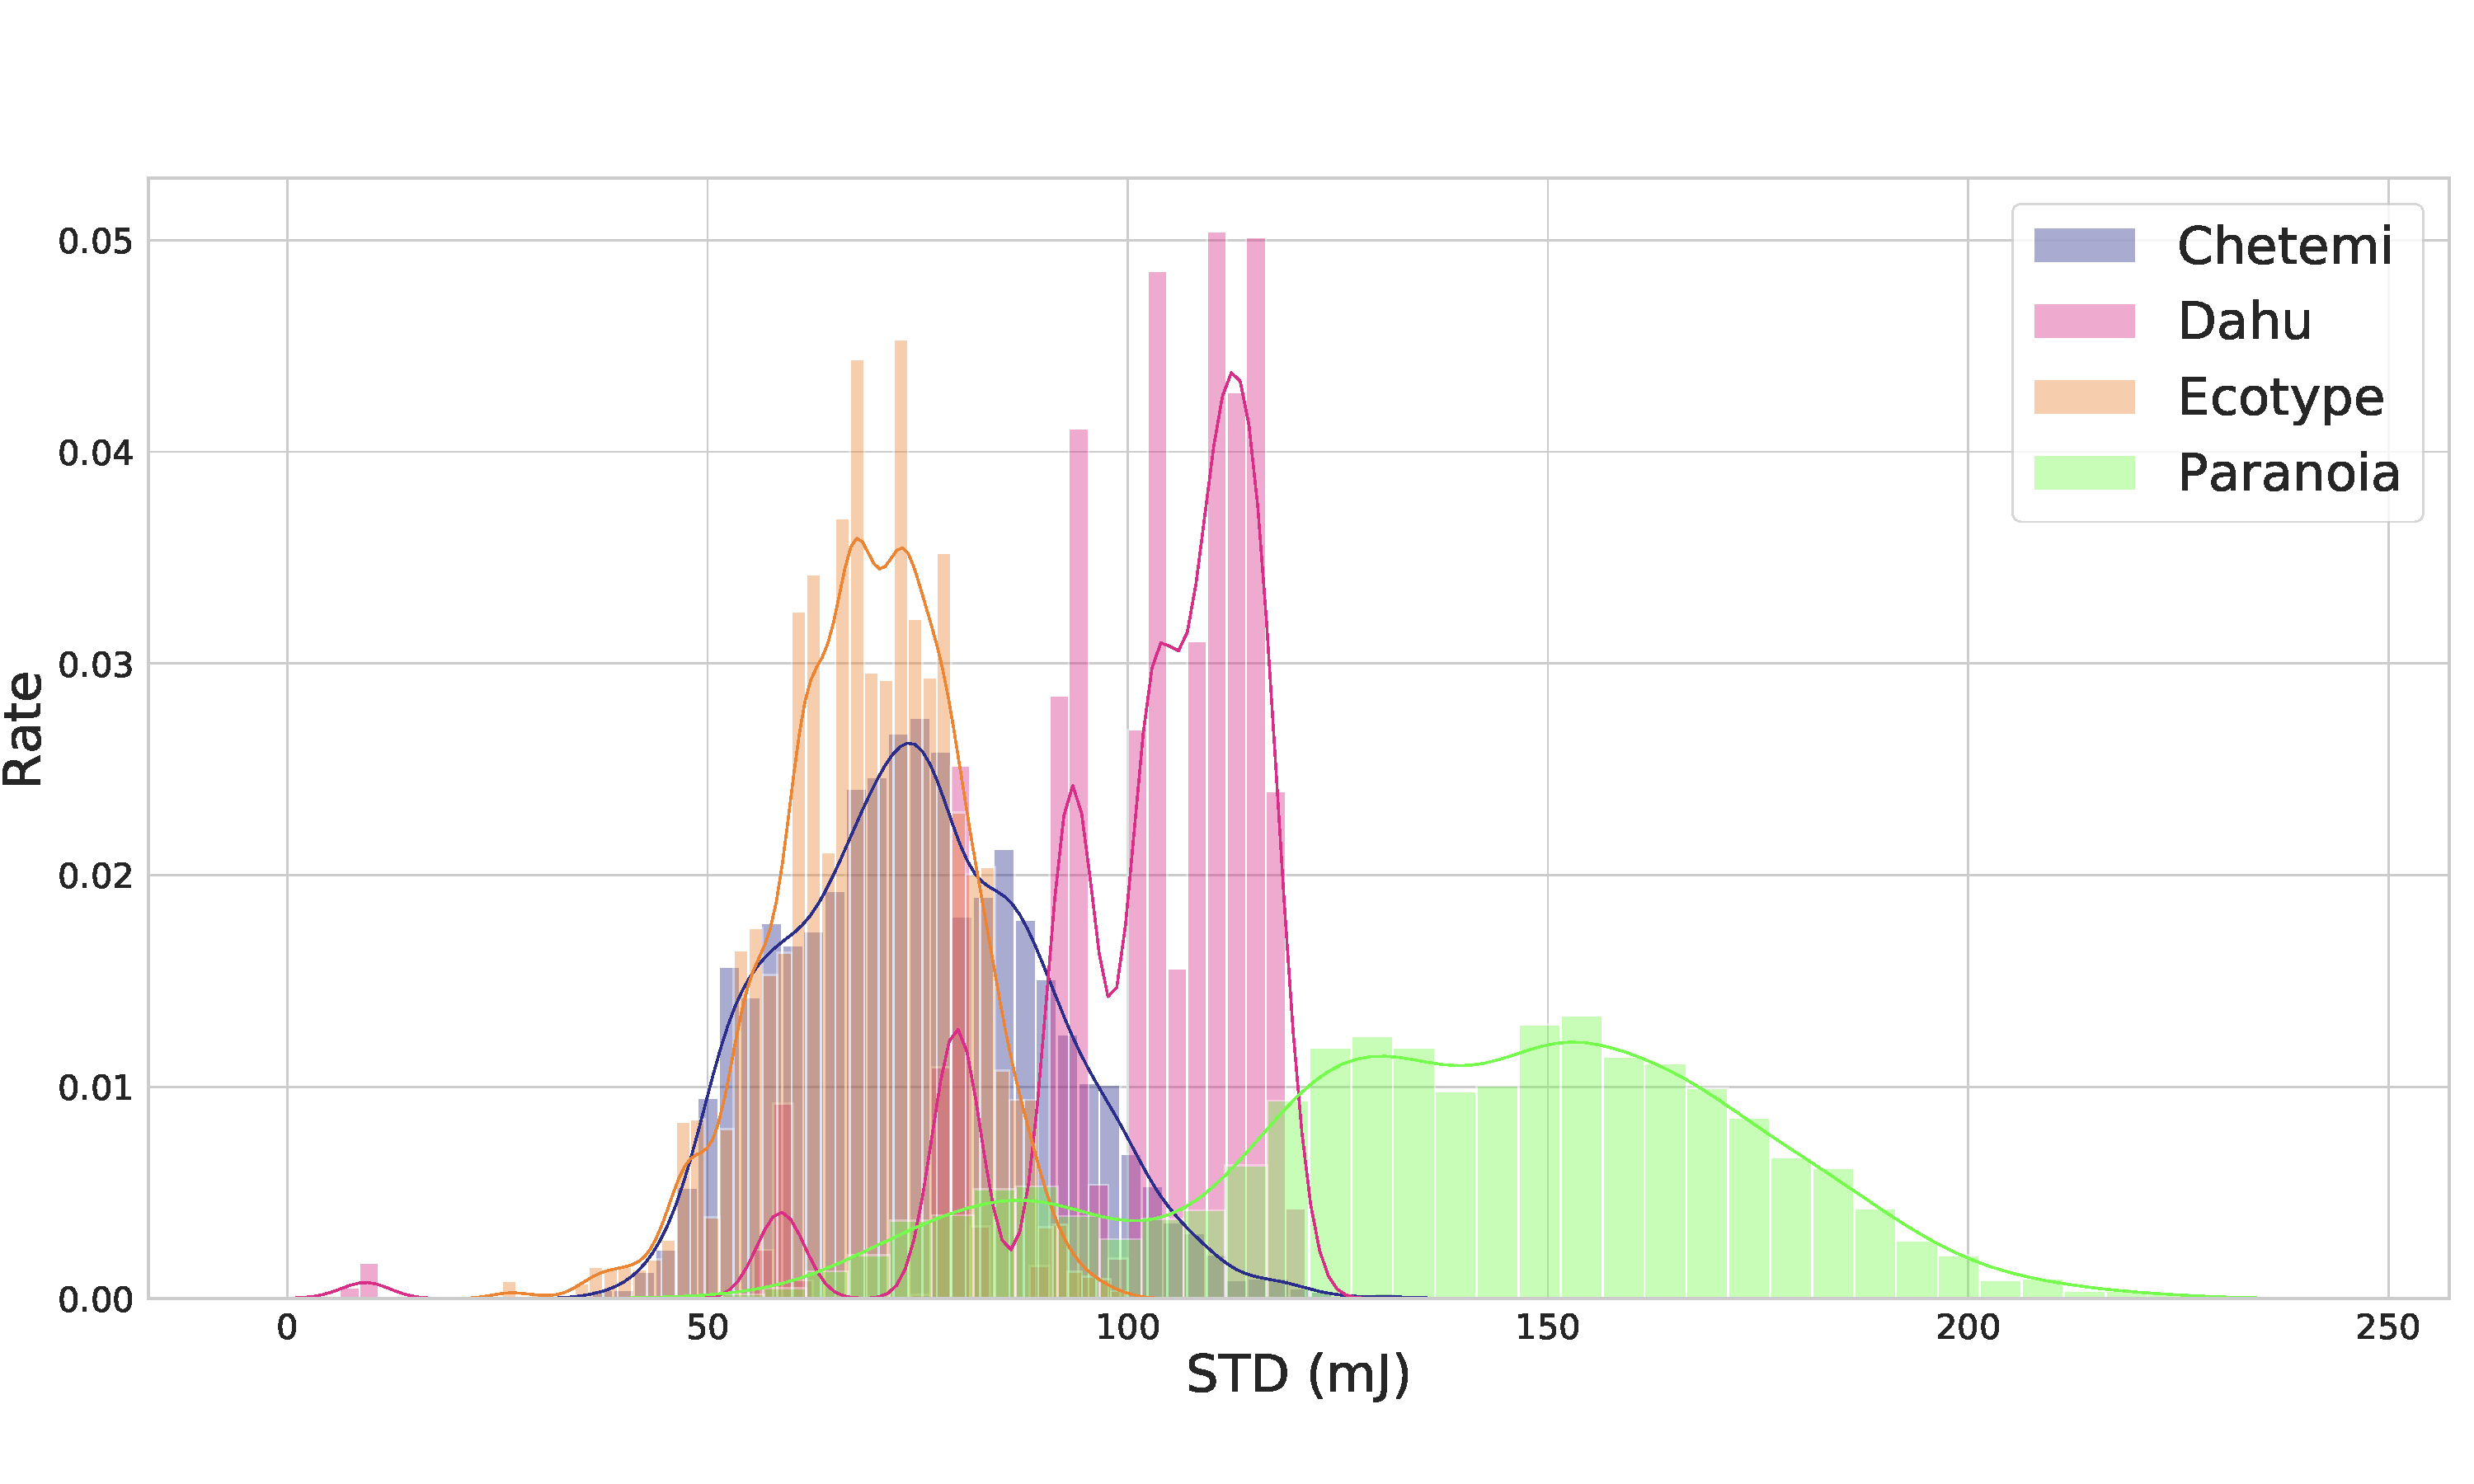
\includegraphics[width=.9\linewidth]{imgs/cpugen}}
    \caption{Energy consumption STD density of the 4 clusters}\label{fig:cpugen}
\end{figure}

\begin{mdframed}[skipabove=\topsep,skipbelow=\topsep]
    We conclude on \textbf{affirming \textsc{RQ}~4}, as selecting the right CPU can help to get less variations.
\end{mdframed}

\section{Experimental Guidelines}\label{sec:guidelines}
To summarize our experiments, we provide some experimental guidelines in Table~\ref{table:guidelines}, based on the multiple experiments and analysis we did.
These guidelines constitute a set of minimal requirements or best practices, depending on the workload and the criticality of the energy measurement precision.
It therefore intends to help practitioners in taming the energy variation on the selected CPU, and conduct the experiments with the least variations.

\begin{table}[h!]
    \centering
    \caption{Experimental Guidelines for Energy Variations}
    \small
    \begin{tabular}{|p{4.7cm}|c|c|}
        \hline
        \textbf{Guideline}                                                                                                                                                & \textbf{Load} & \textbf{Gain}     \\
        \hline
        \hline
        Use a low TDP CPU                                                                                                                                                 & Low \& medium & Up to $3\times$   \\
        \hline
        Disable the CPU C-states                                                                                                                                          & Low           & Up to $6\times$   \\
        \hline
        Use the least of sockets in a case of multiple CPU                                                                                                                & Medium        & Up to $30\times$  \\
        \hline
        Avoid the usage of hyper-threading whenever possible                                                                                                              & Medium        & Up to $5\times$   \\
        \hline
        Avoid rebooting the machine between tests                                                                                                                         & High          & Up to $1.5\times$ \\
        \hline
        Do not relate to the machine idle variation to isolate a test EC, the CPU/OS changes its behavior when a test is running and can exhibit less variation than idle & Any           & ---               \\
        \hline
        Rather focus the optimization efforts on the system under test than the OS                                                                                        & Any           & ---               \\
        \hline
        Execute all the similar and comparable experiments on a same machine. Identical machines can exhibit many differences regarding their energy behavior             & Any           & Up to $1.3\times$ \\
        \hline
    \end{tabular}
    \label{table:guidelines}
\end{table}

Table~\ref{table:guidelines} gives a proper understanding of known factors, like the C-states and its variation reduction at low workloads.
However, it also lists some new factors that we identified along the analysis we conducted in Section~\ref{sec:parameters}, such as the results related to the OS or the reboot mode.
Some of the guidelines are more useful/efficient for specific workloads, as showed in our experiments.
Thus, qualifying the workload before conducting the experiments can help in choosing the proper guidelines to apply.
Other studied factors are not been mentioned in the guidelines, like the Turbo~Boost or the Speculative execution, due to the small effect that has been observed in our study.

In order to validate the accuracy of our guidelines among a varied set of benchmarks on one hand, and their effect on the variation between identical machines on the other hand, we ran seven experiments with benchmarks and real applications on a set of four identical nodes from the cluster \textsf{Dahu}, before (\textsf{normal} mode where everything is left to default and to the charge of the OS) and after (\textsf{optimized}) applying our guidelines.
Half of these experiments has been performed at a 50\,\% workload and the other half on single process jobs.
The choice of these two workloads is related to the optimization guidelines that are mainly effective at low and medium workloads.
We note that we used the cluster \textsf{Dahu} over \textsf{Ecotype} to highlight the guidelines effect on the nodes where the variation is susceptible to be higher.

\begin{figure*}%[!htb]
    \center{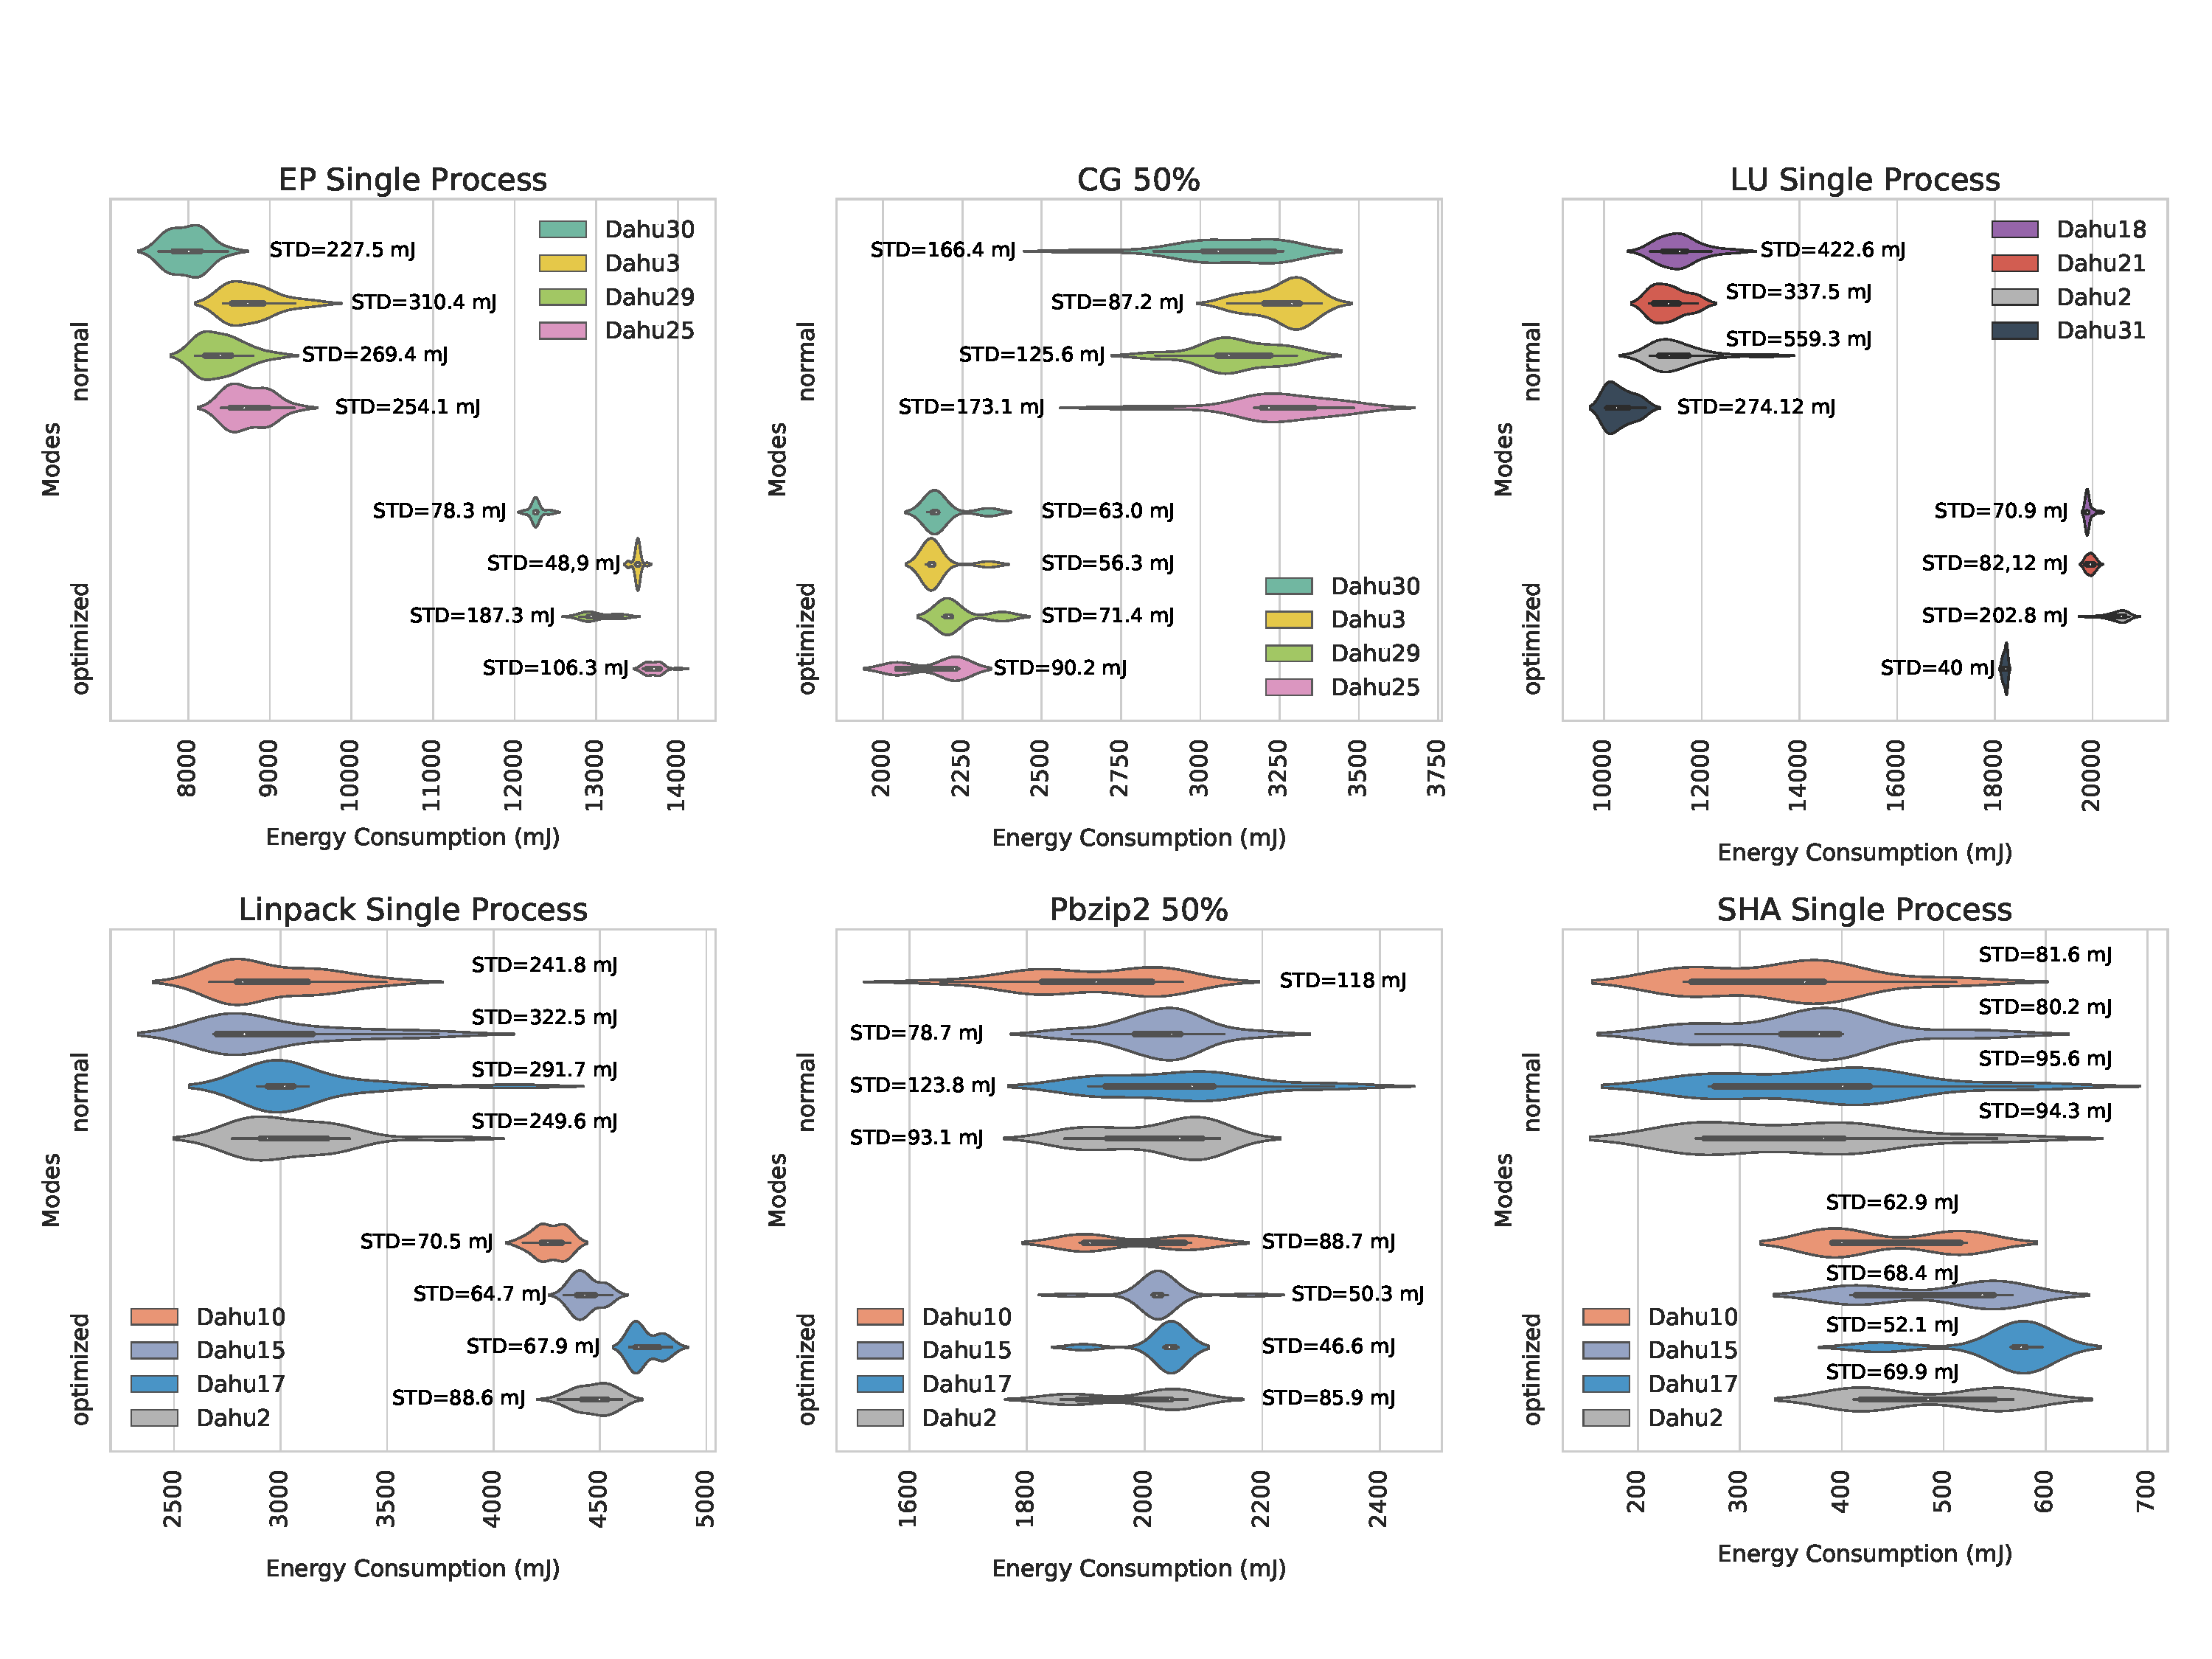
\includegraphics[width=\linewidth]{imgs/all}}
    \caption{Energy variation comparison with/without applying our guidelines}\label{fig:optimized}
\end{figure*}

\begin{figure}%[!htb]
    \center{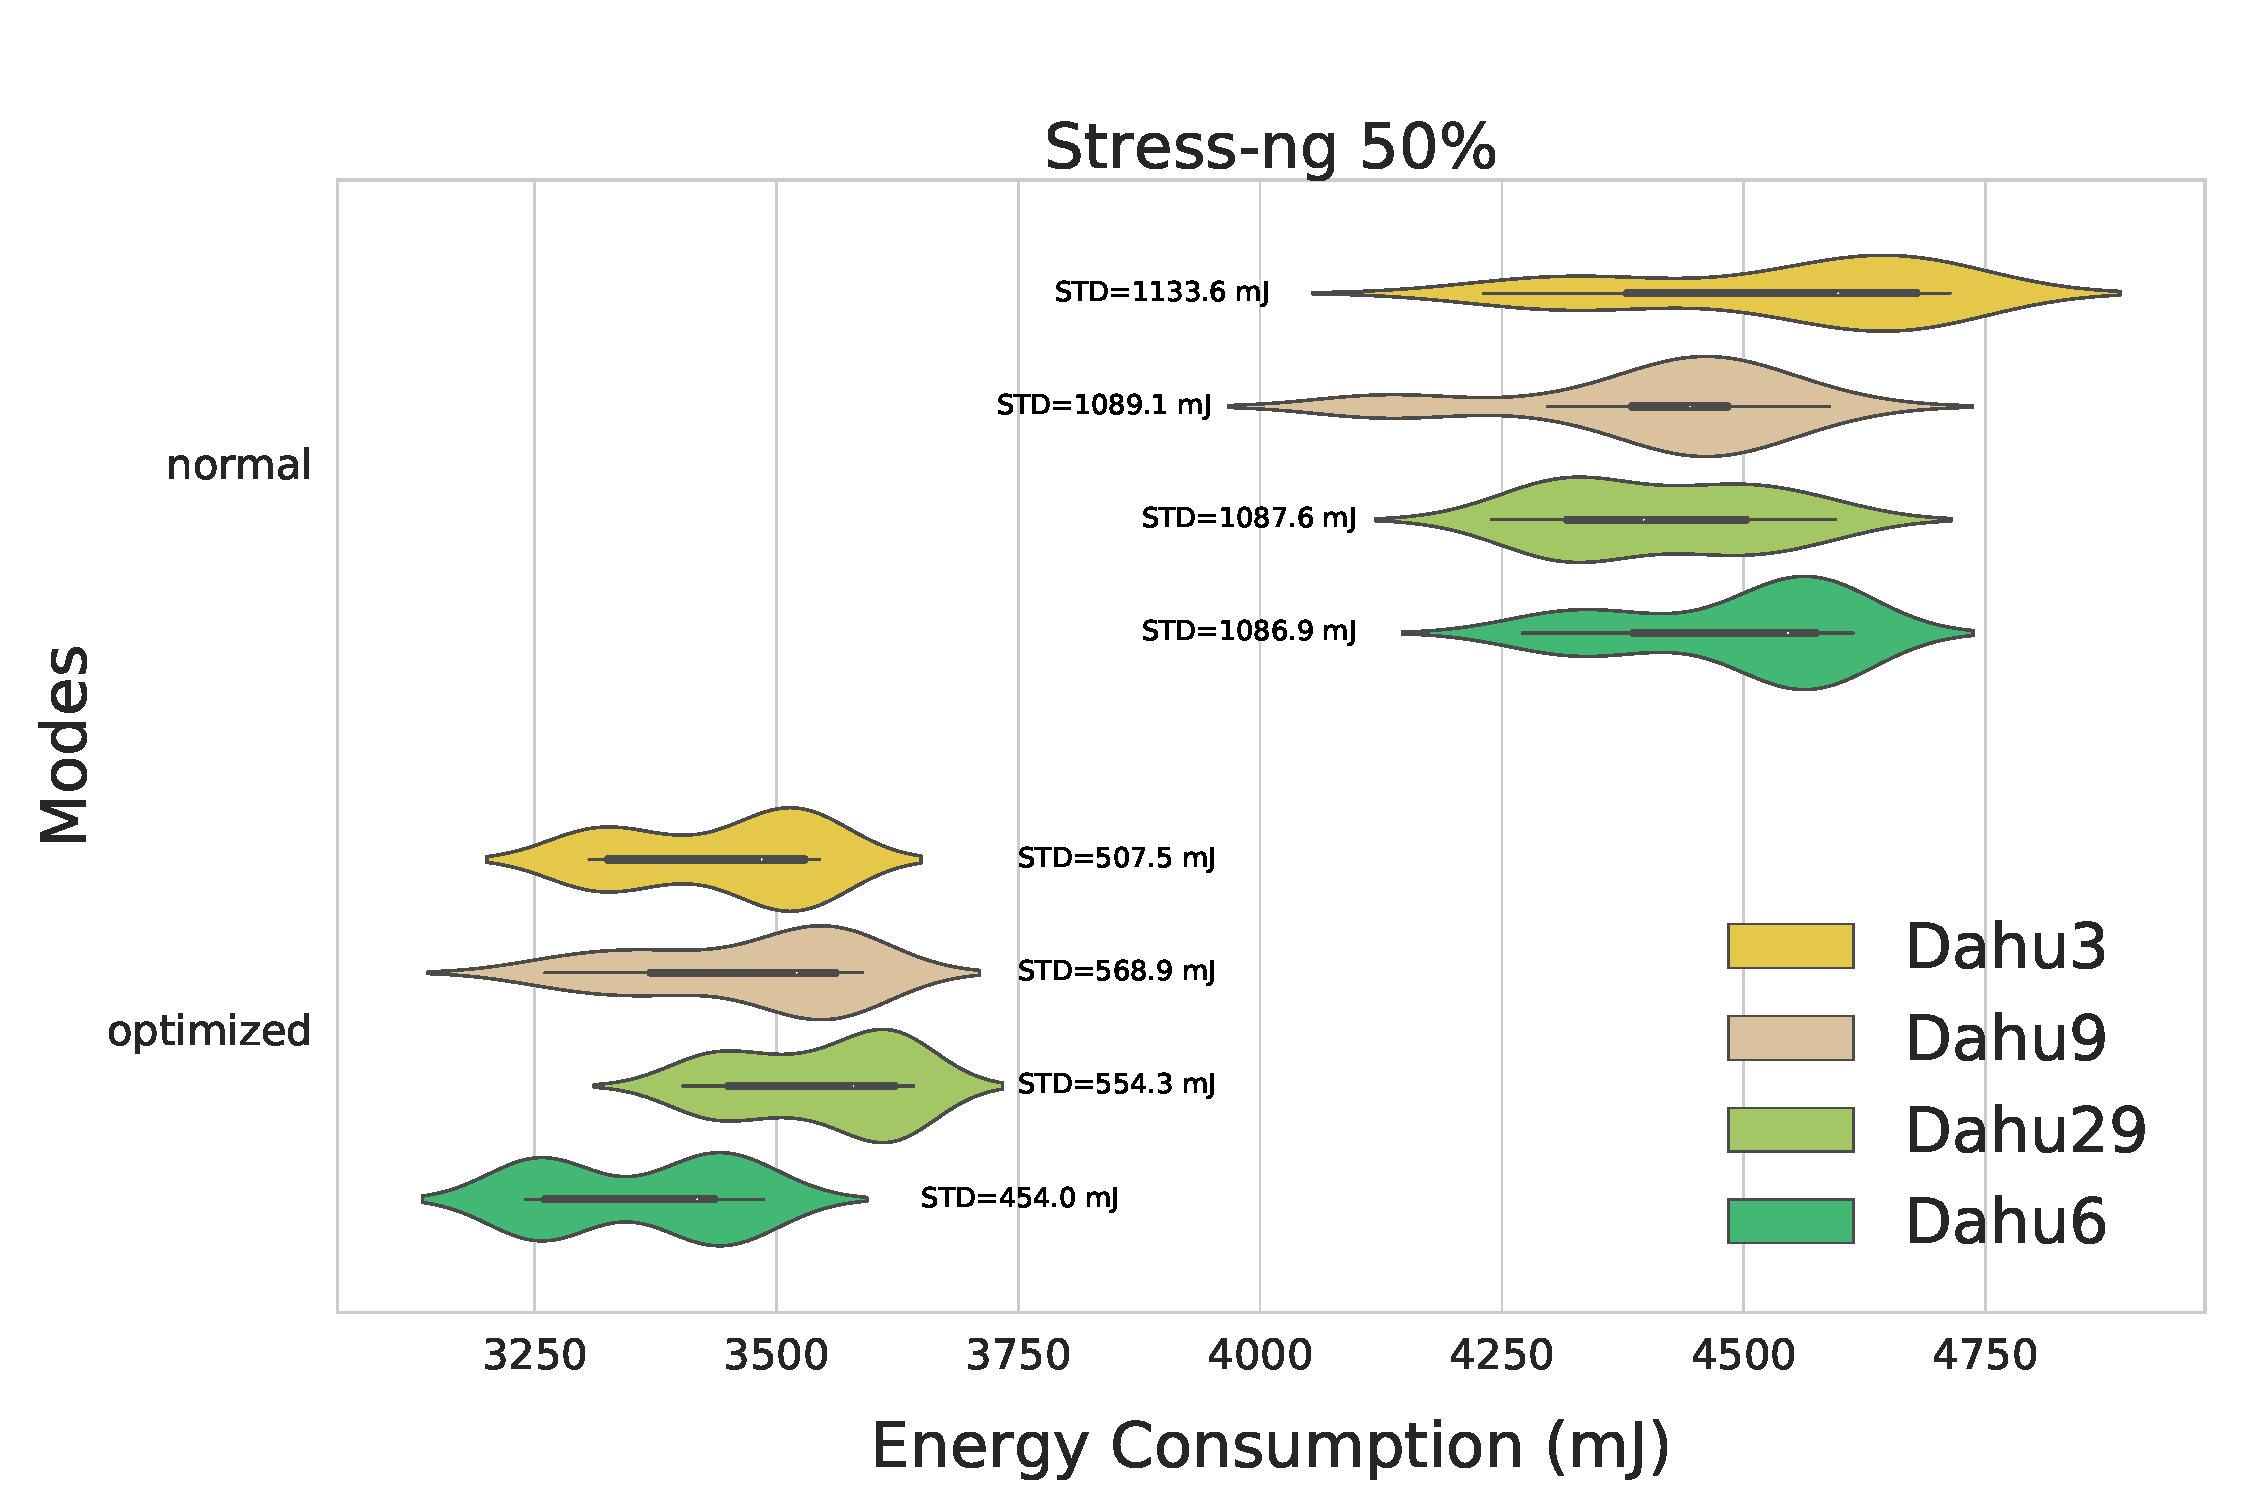
\includegraphics[width=.9\linewidth]{imgs/stressng}}
    \caption{Energy variation comparison with/without applying our guidelines for \textsc{Stress-NG}}\label{fig:stress}
\end{figure}

Figure~\ref{fig:optimized} and~\ref{fig:stress} highlight the improvement brought by the adoption of our guidelines.
They demonstrate the intra-node STD reduction at low and medium workloads for all the benchmarks used at different levels.
Concretely, for low workloads, the energy variation is 2--6 times lower after applying the optimization guidelines for the benchmarks \textsf{LU} and \textsf{EP}, as well as \textsc{Linpack}, while it is 1.2--1.8 times better for \texttt{Sha256}.
For this workload, the overall energy consumption after optimization can be up to 80\,\% higher due to disabling the C-states to keep all the unused cores at a high power consumption state ($Mean_{LU-normal-Dahu2}=11,500 mJ$, $Mean_{LU-optimized-Dahu2}=20,508 mJ$).
For medium workloads, the STD, and thus variation, is up to 100\,\% better for the benchmark \textsf{CG}, 20--150\,\% better for the \texttt{pbzip2} application and up to 100\% for \textsc{Stress-NG}.
We note that the optimized version consumes less energy thanks to an appropriate core pinning method.

Figures~\ref{fig:optimized} and~\ref{fig:stress} also highlight that applying the guidelines does not reduce the inter-nodes variation in all the cases.
This variation can be up to 30\,\% in modern CPU~\cite{wang_experimental_nodate}.
However, taming the intra-node variation is a good strategy to identify more relevant mediums and medians, and then perform accurate comparisons between the nodes variation.
Even though, using the same node is always better, to avoid the extra inter-nodes variation and thus improve the stability of measurements.

\section{Threats to Validity}\label{sec:threats}
A number of issues affect the validity of our work.
For most of our experiments, we used the Intel RAPL tool, which has evolved along Intel CPU generations to be known as one of the most accurate tools for modern CPU, but still adds an important overhead if we adopt a sampling at high frequency.
The other fine-grained tool we used for measurements is \textsc{PowerAPI}.
It allows to measure the energy consumption at the granularity of a process or a Cgroup by dividing the RAPL global energy over the running processes using a power model.
The usage of \textsc{PowerAPI} adds an error margin because of the power model built over RAPL.
The RAPL tool mainly measures the CPU and DRAM energy consumption.
However, even running CPU/RAM intensive benchmarks would keep a degree on uncertainty concerning the hard disk and networking energy consumption.
In addition, the operating system adds a layer of confusion and uncertainty.

The Intel CPU chip manufacturing process and the materials micro-heterogeneity is one of the biggest issues, as we cannot track or justify some of the energy variation between identical CPU or cores.
These CPU/cores might handle frequencies and temperature differently and behave consequently.
This hardware heterogeneity also makes reproduction complex and requires the usage of the same nodes on the cluster with the same OS.

% A more subtle issue may arise due to the values of the measurements that we achieved.
% In fact, the energy measures are quite small, and iterations may be taking a few milliseconds more or less to run.
% A thing we cannot measure using our measurement tools.
% How generalizable are our results? As a set of energy variation optimization guidelines, we argue that our results applied on most of the modern Intel CPU.
% However, using and comparing identical CPU is still tricky and is very dependent to chips.


\section{Conclusion}\label{sec:conclusion}
In this paper, we conducted an empirical study of controllable factors that can increase the energy variations on platforms with some of the latest CPU, and for several workloads.
We provide a set of guidelines that can be implemented and tuned (through the OS GRUB for example), especially with the new data centers isolation trend and the cloud usage, even for scientific and R\&D purposes.
Our guidelines aim at helping the user in reducing the CPU energy variation during systems benchmarking, and conduct more stable experiments when the variation is critical.
For example, when comparing the energy consumption of two versions of an algorithm or a software system, where the difference can be tight and need to be measured accurately.

Overall, our results are not intended to nullify the variability of the CPU, as some of this variability is related to the chip manufacturing process and its thermal behavior.
The aim of our work is to be able to tame and mitigate this variability along controlled experiments.
We studied some previously discussed aspects on some recent CPU, considered new factors that have not been deeply analyzed to the best of our knowledge, and constituted a set of guidelines to achieve the variability mitigating purpose.
Some of these factors, like the C-states usage, can reduce the energy variation up to 500\,\% at low workloads, while choosing the wrong cores/PU strategy can cause up to $30\times$ more variability.

We believe that our approach can also be used to study/discover other potential variability factors, and extend our results to alternative CPU generations/brands.
Most importantly, this should motivate future works on creating a better knowledge on the variability due to CPU manufacturing process and other factors.


\subsection{Testing Protocol}
the results of this protocil can be found in the project of the continious integrtation that was made by the intern Mamadou to give a feedback about the evolution of the energyconsumption within time

